%%%%%%%%%%%%%%%%%%%%%%%%%%%%%%%%%%%
%RSC Article Template with Section Structure
%%%%%%%%%%%%%%%%%%%%%%%%%%%%%%%%%%%

\documentclass[twoside,twocolumn,9pt,fleqn]{article}
\usepackage{extsizes}
\usepackage[super,sort&compress,comma]{natbib}
\usepackage[version=3]{mhchem}
\usepackage[left=1.5cm, right=1.5cm, top=1.785cm, bottom=2.0cm]{geometry}
\usepackage{soul}
\usepackage{balance}
\usepackage{mathptmx}
\usepackage{siunitx}
% Compact E-style scientific notation (1.00000e20) instead of 1.00000 x 10^20.
\sisetup{output-exponent-marker=\text{e}}
\usepackage{sectsty}
\usepackage{graphicx}
\usepackage{lastpage}
\usepackage[format=plain,justification=justified,singlelinecheck=false,font={stretch=1.125,small,sf},labelfont=bf,labelsep=space]{caption}
\usepackage{float}
\usepackage{fancyhdr}
\usepackage{fnpos}
\usepackage[english]{babel}
\usepackage{array}
\usepackage{droidsans}
\usepackage{charter}
\usepackage[T1]{fontenc}
\usepackage[usenames,dvipsnames]{xcolor}
\usepackage{colortbl} % \rowcolor for highlighting table rows
\usepackage{setspace}
\usepackage[compact]{titlesec}
\usepackage{hyperref}
\usepackage[nobreak=false]{mdframed}
\allowdisplaybreaks
\usepackage{makecell}
\usepackage{enumitem}
\usepackage{amssymb}
\usepackage{amsmath}
\usepackage{mathtools}
\usepackage{booktabs}
%\mathtoolsset{showonlyrefs}

\usepackage{epstopdf}%This line makes .eps figures into .pdf - please comment if not required.

\definecolor{cream}{RGB}{222,217,201}

\begin{document}

\pagestyle{fancy}
\thispagestyle{plain}
\fancypagestyle{plain}{
%%%HEADER%%%
\renewcommand{\headrulewidth}{0pt}
}
%%%END OF HEADER%%%

%%%PAGE SETUP - Please do not change any commands within this section%%%
\makeFNbottom
\makeatletter
\renewcommand\LARGE{\@setfontsize\LARGE{15pt}{17}}
\renewcommand\Large{\@setfontsize\Large{12pt}{14}}
\renewcommand\large{\@setfontsize\large{10pt}{12}}
\renewcommand\footnotesize{\@setfontsize\footnotesize{7pt}{10}}
\makeatother

\renewcommand{\thefootnote}{\fnsymbol{footnote}}
\renewcommand\footnoterule{\vspace*{1pt}%
\color{cream}\hrule width 3.5in height 0.4pt \color{black}\vspace*{5pt}}
\setcounter{secnumdepth}{5}

\makeatletter
\renewcommand\@biblabel[1]{[#1]}
\renewcommand\@makefntext[1]%
{\noindent\makebox[0pt][r]{\@thefnmark\,}#1}
\makeatother
\renewcommand{\figurename}{\small{Fig.}~}
\sectionfont{\sffamily\Large}
\subsectionfont{\normalsize}
\subsubsectionfont{\bf}
\setstretch{1.125} %In particular, please do not alter this line.
\setlength{\skip\footins}{0.4cm}
\setlength{\footnotesep}{0.25cm}
\setlength{\jot}{3pt}
\setlength{\mathindent}{1.5em}
\titlespacing*{\section}{0pt}{4pt}{4pt}
\titlespacing*{\subsection}{0pt}{15pt}{1pt}
\raggedbottom % keep inter-paragraph spacing uniform; do not stretch columns to fill the page
%%%END OF PAGE SETUP%%%

%%%FOOTER%%%
\fancyfoot{}
\fancyfoot[LO,RE]{\vspace{-7.1pt}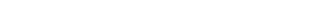
\includegraphics[height=9pt]{head_foot/LF}}
%\fancyfoot[CO]{\vspace{-7.1pt}\hspace{11.9cm}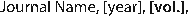
\includegraphics{head_foot/RF}}
%\fancyfoot[CE]{\vspace{-7.2pt}\hspace{-13.2cm}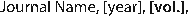
\includegraphics{head_foot/RF}}
\fancyfoot[RO]{\footnotesize{\sffamily{1--\pageref{LastPage} ~\textbar  \hspace{2pt}\thepage}}}
\fancyfoot[LE]{\footnotesize{\sffamily{\thepage~\textbar\hspace{4.65cm} 1--\pageref{LastPage}}}}
\fancyhead{}
\renewcommand{\headrulewidth}{0pt}
\renewcommand{\footrulewidth}{0pt}
\setlength{\arrayrulewidth}{1pt}
\setlength{\columnsep}{6.5mm}
\setlength\bibsep{1pt}
%%%END OF FOOTER%%%

%%%FIGURE SETUP - please do not change any commands within this section%%%
\makeatletter
\newlength{\figrulesep}
\setlength{\figrulesep}{0.5\textfloatsep}

\newcommand{\topfigrule}{\vspace*{-1pt}%
\noindent{\color{cream}\rule[-\figrulesep]{\columnwidth}{1.5pt}} }

\newcommand{\botfigrule}{\vspace*{-2pt}%
\noindent{\color{cream}\rule[\figrulesep]{\columnwidth}{1.5pt}} }

\newcommand{\dblfigrule}{\vspace*{-1pt}%
\noindent{\color{cream}\rule[-\figrulesep]{\textwidth}{1.5pt}} }

\makeatother
%%%END OF FIGURE SETUP%%%

%%%TITLE, AUTHORS AND ABSTRACT%%%
\twocolumn[
  \begin{@twocolumnfalse}

  {  \noindent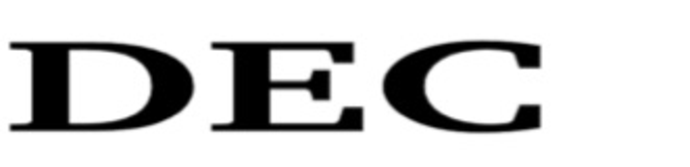
\includegraphics[height=30pt]{head_foot/dec}}\\
  \normalsize\text{DOI: \href{https://doi.org/10.5281/zenodo.21222282}{10.5281/zenodo.21222282}}
{\hfill\raisebox{0pt}[0pt][0pt]{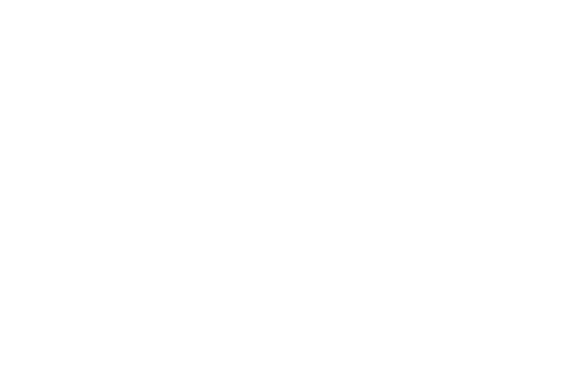
\includegraphics[height=55pt]{head_foot/RSC_LOGO_CMYK}}\\[1ex]
}\par
\vspace{1em}
\sffamily
\begin{tabular}{m{4.5cm} p{13.5cm} }

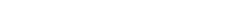
\includegraphics{head_foot/DOI} & \noindent\LARGE{\textbf{Explaining the Relative Nature of General and Special Relativity}} \\
\vspace{0.3cm} & \vspace{0.3cm} \\
 & \noindent\large{Thomas DeGerlia\textit{$^{a}$}} \\
 & \noindent\small{Originally published: July 4, 2026 C.E.\textit{$^{b}$}} \\
 & \noindent\small{Revision 6 July 18, 2026 C.E.} \\
 & \noindent\small{OPEN RESEARCH PREPRINT - FOR PEER REVIEW} \\
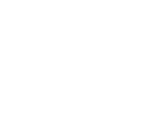
\includegraphics{head_foot/dates} & \\
 & \vspace{0.3cm} \\
 & \noindent\normalsize{ABSTRACT: In this paper, we show that time dilation is not a property of a single system but a comparison between two systems, defined solely by their relative spatial distribution of mass. Specifically stated, the time dilation between two systems is governed by the relative DeGerlia Inertial Density $D$, defined as mass divided by mean radius about the compared axis. We first exemplify this comparative nature with one of the most fundamental equivalences in General Relativity, the gravitational time-dilation equation, which computes a system's time dilation relative to flat spacetime: $d\tau/dt = \sqrt{1 - r_{\mathrm{s}}/r}$. We use this reference value to validate the calculation we perform using relative $D$ alone. We then validate correct calculations for a diverse set of two-system examples, including transformed systems (similar to the gravitational time dilation above, where system 2 is a transformed version of system 1) as well as discrete system comparisons, across the classical and relativistic regimes. To conduct this demonstration, we introduce the DeGerlia Time Dilation Framework (DTDF), a simple, mathematically equivalent framework, fully defined by general relativity, that offers a second frame for visualizing the relative nature of time.} \\
 & \vspace{0.15cm} \\
 & \noindent\small{\textbf{Keywords:} time dilation, general relativity, special relativity, gravitational time dilation, Lorentz time dilation, DeGerlia inertial density, inertial density, moment of inertia, astrophysics, Schwarzschild radius, DTDF, DTD, degerlia time dilation} \\
\end{tabular}

 \end{@twocolumnfalse} \vspace{0.6cm}

  ]
%%%END OF TITLE, AUTHORS AND ABSTRACT%%%

%%%FONT SETUP - please do not change any commands within this section
\renewcommand*\rmdefault{bch}\normalfont\upshape
\rmfamily
\vspace{-1cm}
%%%FOOTNOTES%%%
\footnotetext{$^{a}$~DeGerlia Expert Consulting, 3000 Lawrence Street, Denver, CO, United States of America. E-mail: tom.degerlia@tomdegerlia.com}
\footnotetext{$^{b}$~This paper was originally published on July 4, 2026, the quarter-millennial anniversary of the Declaration of Independence of the United States of America.}
% Auto-generated full pair comparison tables
\begin{table*}[t]
\footnotesize\centering
\setlength{\tabcolsep}{4pt}
\caption{System properties for each pair comparison case (six significant figures; GTD in $1-\delta$ form).}\label{tab:pair_properties}
\begin{tabular}{lrrrrrr}
\toprule
 & Case 1 ($M{=}M$) & Case 2 ($R{=}R$) & Case 3 ($\rho{=}\rho$) & Case 4 ($I{=}I$) & General & Classical \\
\midrule
$m_1$ (kg) & $2.00000\times10^{30}$ & $1.00000\times10^{30}$ & $1.00000\times10^{30}$ & $1.00000\times10^{32}$ & $1.00000\times10^{20}$ & $8.00000\times10^{0}$ \\
$m_2$ (kg) & $2.00000\times10^{30}$ & $1.00000\times10^{24}$ & $1.00000\times10^{27}$ & $1.00000\times10^{30}$ & $1.00000\times10^{30}$ & $1.00000\times10^{0}$ \\
$R_1$ (m) & $3.00000\times10^{3}$ & $1.00000\times10^{8}$ & $1.00000\times10^{8}$ & $1.00000\times10^{7}$ & $2.00000\times10^{-7}$ & $2.00000\times10^{0}$ \\
$R_2$ (m) & $7.00000\times10^{8}$ & $1.00000\times10^{8}$ & $1.00000\times10^{7}$ & $1.00000\times10^{8}$ & $1.00000\times10^{7}$ & $1.00000\times10^{0}$ \\
$\rho_1$ (kg/m$^3$) & $1.76839\times10^{19}$ & $2.38732\times10^{5}$ & $2.38732\times10^{5}$ & $2.38732\times10^{10}$ & $2.98416\times10^{39}$ & $2.38732\times10^{-1}$ \\
$\rho_2$ (kg/m$^3$) & $1.39203\times10^{3}$ & $2.38732\times10^{-1}$ & $2.38732\times10^{5}$ & $2.38732\times10^{5}$ & $2.38732\times10^{8}$ & $2.38732\times10^{-1}$ \\
$I_1$ (kg\,m$^2$) & $7.20000\times10^{36}$ & $4.00000\times10^{45}$ & $4.00000\times10^{45}$ & $4.00000\times10^{45}$ & $1.60000\times10^{6}$ & $1.28000\times10^{1}$ \\
$I_2$ (kg\,m$^2$) & $3.92000\times10^{47}$ & $4.00000\times10^{39}$ & $4.00000\times10^{40}$ & $4.00000\times10^{45}$ & $4.00000\times10^{43}$ & $4.00000\times10^{-1}$ \\
$D_1$ (kg/m) & $6.66667\times10^{26}$ & $1.00000\times10^{22}$ & $1.00000\times10^{22}$ & $1.00000\times10^{25}$ & $5.00000\times10^{26}$ & $4.00000\times10^{0}$ \\
$D_2$ (kg/m) & $2.85714\times10^{21}$ & $1.00000\times10^{16}$ & $1.00000\times10^{20}$ & $1.00000\times10^{22}$ & $1.00000\times10^{23}$ & $1.00000\times10^{0}$ \\
$r_{s,1}$ (m) & $2.97046\times10^{3}$ & $1.48523\times10^{3}$ & $1.48523\times10^{3}$ & $1.48523\times10^{5}$ & $1.48523\times10^{-7}$ & $1.18819\times10^{-26}$ \\
$r_{s,2}$ (m) & $2.97046\times10^{3}$ & $1.48523\times10^{-3}$ & $1.48523\times10^{0}$ & $1.48523\times10^{3}$ & $1.48523\times10^{3}$ & $1.48523\times10^{-27}$ \\
$k_{s,1}$ & $9.90155\times10^{-1}$ & $1.48523\times10^{-5}$ & $1.48523\times10^{-5}$ & $1.48523\times10^{-2}$ & $7.42616\times10^{-1}$ & $5.94093\times10^{-27}$ \\
$k_{s,2}$ & $4.24352\times10^{-6}$ & $1.48523\times10^{-11}$ & $1.48523\times10^{-7}$ & $1.48523\times10^{-5}$ & $1.48523\times10^{-4}$ & $1.48523\times10^{-27}$ \\
$k_{d,1}$ & $9.90155\times10^{-1}$ & $1.48523\times10^{-5}$ & $1.48523\times10^{-5}$ & $1.48523\times10^{-2}$ & $7.42617\times10^{-1}$ & $5.94093\times10^{-27}$ \\
$k_{d,2}$ & $4.24352\times10^{-6}$ & $1.48523\times10^{-11}$ & $1.48523\times10^{-7}$ & $1.48523\times10^{-5}$ & $1.48523\times10^{-4}$ & $1.48523\times10^{-27}$ \\
$\mathrm{DTD}_1$ & $9.95066\times10^{-1}$ & $3.85387\times10^{-3}$ & $3.85387\times10^{-3}$ & $1.21870\times10^{-1}$ & $8.61752\times10^{-1}$ & $7.70774\times10^{-14}$ \\
$\mathrm{DTD}_2$ & $2.05998\times10^{-3}$ & $3.85387\times10^{-6}$ & $3.85387\times10^{-4}$ & $3.85387\times10^{-3}$ & $1.21870\times10^{-2}$ & $3.85387\times10^{-14}$ \\
$\mathrm{GTD}_{s,1}$ & $1-9.00777\times10^{-1}$ & $1-7.42619\times10^{-6}$ & $1-7.42619\times10^{-6}$ & $1-7.45394\times10^{-3}$ & $1-4.92670\times10^{-1}$ & $1-2.97046\times10^{-27}$ \\
$\mathrm{GTD}_{s,2}$ & $1-2.12176\times10^{-6}$ & $1-7.42616\times10^{-12}$ & $1-7.42616\times10^{-8}$ & $1-7.42619\times10^{-6}$ & $1-7.42644\times10^{-5}$ & $1-7.42616\times10^{-28}$ \\
$\mathrm{GTD}_{d,1}$ & $1-9.00780\times10^{-1}$ & $1-7.42619\times10^{-6}$ & $1-7.42619\times10^{-6}$ & $1-7.45395\times10^{-3}$ & $1-4.92670\times10^{-1}$ & $1-2.97047\times10^{-27}$ \\
$\mathrm{GTD}_{d,2}$ & $1-2.12176\times10^{-6}$ & $1-7.42617\times10^{-12}$ & $1-7.42617\times10^{-8}$ & $1-7.42619\times10^{-6}$ & $1-7.42644\times10^{-5}$ & $1-7.42617\times10^{-28}$ \\
\bottomrule
\end{tabular}
\end{table*}

\begin{table*}[t]
\footnotesize\centering
\setlength{\tabcolsep}{4pt}
\caption{Derived ratios across constraint cases. Group A is the DTD ratio; Group B the $k$-ratio; Group C the GTD ratio by both routes; Groups D and E the inertia/density and component analogs.}\label{tab:pair_ratios}
\begin{tabular}{lrrrrrr}
\toprule
 & Case 1 ($M{=}M$) & Case 2 ($R{=}R$) & Case 3 ($\rho{=}\rho$) & Case 4 ($I{=}I$) & General & Classical \\
\midrule
\multicolumn{7}{l}{\textit{Group A --- DTD ratio}}\\
$\mathrm{DTD}_1/\mathrm{DTD}_2$ & $4.83046\times10^{2}$ & $1.00000\times10^{3}$ & $1.00000\times10^{1}$ & $3.16228\times10^{1}$ & $7.07107\times10^{1}$ & $2.00000\times10^{0}$ \\
$\sqrt{D_1/D_2}$ & $4.83046\times10^{2}$ & $1.00000\times10^{3}$ & $1.00000\times10^{1}$ & $3.16228\times10^{1}$ & $7.07107\times10^{1}$ & $2.00000\times10^{0}$ \\
$\sqrt{M_1 R_2/(M_2 R_1)}$ & $4.83046\times10^{2}$ & $1.00000\times10^{3}$ & $1.00000\times10^{1}$ & $3.16228\times10^{1}$ & $7.07107\times10^{1}$ & $2.00000\times10^{0}$ \\
$\sqrt{(I_1/I_2)(R_2/R_1)^3}$ & $4.83046\times10^{2}$ & $1.00000\times10^{3}$ & $1.00000\times10^{1}$ & $3.16228\times10^{1}$ & $7.07107\times10^{1}$ & $2.00000\times10^{0}$ \\
$(I_1/I_2)^{1/5}(\rho_1/\rho_2)^{3/10}$ & $4.83046\times10^{2}$ & $1.00000\times10^{3}$ & $1.00000\times10^{1}$ & $3.16228\times10^{1}$ & $7.07107\times10^{1}$ & $2.00000\times10^{0}$ \\
\midrule
\multicolumn{7}{l}{\textit{Group B --- $k$-ratio}}\\
$D_1/D_2$ & $2.33333\times10^{5}$ & $1.00000\times10^{6}$ & $1.00000\times10^{2}$ & $1.00000\times10^{3}$ & $5.00000\times10^{3}$ & $4.00000\times10^{0}$ \\
$M_1 R_2/(M_2 R_1)$ & $2.33333\times10^{5}$ & $1.00000\times10^{6}$ & $1.00000\times10^{2}$ & $1.00000\times10^{3}$ & $5.00000\times10^{3}$ & $4.00000\times10^{0}$ \\
$(I_1/I_2)(R_2/R_1)^3$ & $2.33333\times10^{5}$ & $1.00000\times10^{6}$ & $1.00000\times10^{2}$ & $1.00000\times10^{3}$ & $5.00000\times10^{3}$ & $4.00000\times10^{0}$ \\
$D_2/D_1$ & $4.28571\times10^{-6}$ & $1.00000\times10^{-6}$ & $1.00000\times10^{-2}$ & $1.00000\times10^{-3}$ & $2.00000\times10^{-4}$ & $2.50000\times10^{-1}$ \\
$M_2 R_1/(M_1 R_2)$ & $4.28571\times10^{-6}$ & $1.00000\times10^{-6}$ & $1.00000\times10^{-2}$ & $1.00000\times10^{-3}$ & $2.00000\times10^{-4}$ & $2.50000\times10^{-1}$ \\
\midrule
\multicolumn{7}{l}{\textit{Group C --- GTD ratio}}\\
$\mathrm{GTD}_{s,1}/\mathrm{GTD}_{s,2}$ & $1-9.00776\times10^{-1}$ & $1-7.42618\times10^{-6}$ & $1-7.35193\times10^{-6}$ & $1-7.44657\times10^{-3}$ & $1-4.92632\times10^{-1}$ & $1-2.22785\times10^{-27}$ \\
$\mathrm{GTD}_{d,1}/\mathrm{GTD}_{d,2}$ & $1-9.00780\times10^{-1}$ & $1-7.42619\times10^{-6}$ & $1-7.35193\times10^{-6}$ & $1-7.44658\times10^{-3}$ & $1-4.92633\times10^{-1}$ & $1-2.22785\times10^{-27}$ \\
\midrule
\multicolumn{7}{l}{\textit{Group D --- inertia and density analogs}}\\
$I_1/I_2$ & $1.83673\times10^{-11}$ & $1.00000\times10^{6}$ & $1.00000\times10^{5}$ & $1.00000\times10^{0}$ & $4.00000\times10^{-38}$ & $3.20000\times10^{1}$ \\
$(I_1/I_2)^{1/2}$ & $4.28571\times10^{-6}$ & $1.00000\times10^{3}$ & $3.16228\times10^{2}$ & $1.00000\times10^{0}$ & $2.00000\times10^{-19}$ & $5.65685\times10^{0}$ \\
$(I_1/I_2)^{1/5}$ & $7.12540\times10^{-3}$ & $1.58489\times10^{1}$ & $1.00000\times10^{1}$ & $1.00000\times10^{0}$ & $3.31445\times10^{-8}$ & $2.00000\times10^{0}$ \\
$(\rho_1/\rho_2)^{1/5}(R_1/R_2)$ & $7.12540\times10^{-3}$ & $1.58489\times10^{1}$ & $1.00000\times10^{1}$ & $1.00000\times10^{0}$ & $3.31445\times10^{-8}$ & $2.00000\times10^{0}$ \\
$(\mathrm{DTD}_1/\mathrm{DTD}_2)^2(R_1/R_2)^3$ & $1.83673\times10^{-11}$ & $1.00000\times10^{6}$ & $1.00000\times10^{5}$ & $1.00000\times10^{0}$ & $4.00000\times10^{-38}$ & $3.20000\times10^{1}$ \\
\midrule
\multicolumn{7}{l}{\textit{Group E --- component scale factors}}\\
$M_1/M_2$ & $1.00000\times10^{0}$ & $1.00000\times10^{6}$ & $1.00000\times10^{3}$ & $1.00000\times10^{2}$ & $1.00000\times10^{-10}$ & $8.00000\times10^{0}$ \\
$\sqrt{M_1/M_2}$ & $1.00000\times10^{0}$ & $1.00000\times10^{3}$ & $3.16228\times10^{1}$ & $1.00000\times10^{1}$ & $1.00000\times10^{-5}$ & $2.82843\times10^{0}$ \\
$R_1/R_2$ & $4.28571\times10^{-6}$ & $1.00000\times10^{0}$ & $1.00000\times10^{1}$ & $1.00000\times10^{-1}$ & $2.00000\times10^{-14}$ & $2.00000\times10^{0}$ \\
$R_2/R_1$ & $2.33333\times10^{5}$ & $1.00000\times10^{0}$ & $1.00000\times10^{-1}$ & $1.00000\times10^{1}$ & $5.00000\times10^{13}$ & $5.00000\times10^{-1}$ \\
$\sqrt{R_2/R_1}$ & $4.83046\times10^{2}$ & $1.00000\times10^{0}$ & $3.16228\times10^{-1}$ & $3.16228\times10^{0}$ & $7.07107\times10^{6}$ & $7.07107\times10^{-1}$ \\
$\sqrt{M_2^2 R_2/(M_1^2 R_1)}$ & $4.83046\times10^{2}$ & $1.00000\times10^{-6}$ & $3.16228\times10^{-4}$ & $3.16228\times10^{-2}$ & $7.07107\times10^{16}$ & $8.83883\times10^{-2}$ \\
\bottomrule
\end{tabular}
\end{table*}


\section{Introduction}
General Relativity\cite{einstein1915} is a model for describing our universe that is fundamentally comparative: no quantity has physical meaning without a comparator. The pace of time is no exception: the time dilation between two systems is a product of the systems' relative geometric mass distributions. Directly from the gravitational time dilation (GTD) formula, one can derive the underlying two-system logic, and ultimately, GTD is simply a comparison between a system's pace of time relative to the pace of time of a selected benchmark system, which in this case is a system of the same mass, but at its Schwarzschild radius. The formula requires only one mass and one radius, the second system being derived directly from the first. While this is the familiar representation, it obscures the comparative nature of relativity and implies that one need not compare two systems to characterize time. That implication is incorrect: there is no privileged perspective from which to characterize time. In this paper, we evaluate the physical property responsible for relativistic time dilation and explore the underlying formulation that quantifies the relative time dilation between two systems.

The relative flow of time between two systems is governed solely by their relative DeGerlia inertial density $D$. We demonstrate this across a range of uniform spherical systems, from the classical to the relativistic regime, by calculating each system’s DeGerlia time dilation from its relative $D$, converting each to its gravitational time dilation, and taking their ratio. In each case this matches the ratio obtained by computing each system’s gravitational time dilation independently from the standard Schwarzschild form, to the precision permitted by $G$. Given two systems’ masses and radii, their relative time dilation is determined by their relative spatial distribution of mass alone, a relation already contained in general relativity.

\section{Experimental Model}

The experimental model employed in this study comprises several components. The framework is derived directly from general relativity and is mathematically equivalent to established general-relativistic calculations. It neither relies upon nor introduces any principle not already established within the theories of general and special relativity; this paper leverages a framing of the existing theory of relativity for illustrative purposes.

We begin by introducing the DeGerlia Framework and then demonstrate its complete mathematical equivalence with general relativity. We then work through a series of examples, each demonstrating a different comparative case, and in each case, we validate the result using standard gravitational time-dilation calculations.

These examples demonstrate the two-system nature of all relativistic calculations. Relativity is fundamentally concerned with how quantities appear relative to one another; gravitational time dilation, for instance, reflects the comparison of a system with an identical system at its Schwarzschild radius, the collapse-condition radius $r_{\mathrm{s}}$.

\section{The DeGerlia Time Dilation Framework}

\subsection{Definitions, Formulas and Constants Used Herein}

\noindent
\begin{tabular}{@{}l p{6.7cm}@{}}
\toprule
Symbol & Definition / Value \\
\midrule
$c$ & Light Speed $\num{299792458}\,\unit{\meter\per\second}$ \\
$D$ & DeGerlia Inertial Density $m/r$, where $r$ is the mean radius about a selected axis \\
$D_{\mathrm{crit}}$ & DeGerlia Threshold $c^2/2G = \num{6.73295e26}\,\unit[per-mode=symbol]{\kilogram\per\meter}$ \\
DTD & DeGerlia Time Dilation $\sqrt{k}$  \\
$G$ & Gravitational Constant $\num{6.67430e-11} \pm \num{1.5e-15}\,\unit{\meter\cubed\per\kilogram\per\second\squared}$ \\
GTD & Gravitational Time Dilation $d\tau/dt = \sqrt{1-k}$ \\
$k$ & Linear Scale Factor $v^2/c^2=r_{\mathrm{s}}/r=D/D_{\mathrm{crit}}$ \\
$k_{D}$ & Linear Scale Factor (DeGerlia inertial density) $D/D_{\mathrm{crit}}$ \\
$k_{s}$ & Linear Scale Factor (Schwarzschild) $r_{\mathrm{s}}/r$ \\
$k_{v}$ & Linear Scale Factor (velocity) $v^2/c^2$ \\
$P$ & Inertial Density $I/V$ $=D\cdot 3/10\pi$ \\
$r_{\mathrm{s}}$ & Schwarzschild Radius $2Gm/c^2$  \\
\bottomrule
\end{tabular}

\subsection{What is the DeGerlia Time Dilation Framework?}

First and foremost, the entirety of the principles described herein represents no deviation from general relativity. It represents a mathematically equivalent reframing useful in certain relativistic calculations. The author has simply asserted a complement to GTD, where the form of time dilation is equal to $\sqrt{k}$, instead of $\sqrt{1-k}$.

While equivalent to GTD mathematically, the DTD form offers a different perspective on the same physical phenomenon. It is a complementary perspective that aids in visualizing the underlying physics:
\begin{itemize}
\item One can convert between GTD and DTD at any time. GTD is always recoverable.
\item $\mathrm{DTD}$ is mathematically very easy to use and visualize, requiring only the ratio of mass to radius in comparison to a static constant to perform gravitational time dilation calculations. 
\item $\mathrm{DTD}$ allows for direct calculation of time dilation between two systems, without the need to reference a third system (the Schwarzschild condition)
\item $\mathrm{DTD}$ returns finite output over the entire range of finite input.
\item $\mathrm{DTD}$ represents flat spacetime as an ideal state that can only be approached.
\item $\mathrm{DTD}$ represents the Schwarzschild condition as the point where the gravitational escape velocity exceeds the speed of light, and an event horizon forms. While we have observed black holes, the asymptotically approached ideal state of zero time dilation is not attainable.
\item $\mathrm{DTD}$ reflects the singularity state as an asymptotic approach to $r=0$.
\end{itemize}


\subsection{Inertia and Moment of Inertia}
In classical physics, inertia dictates how a system's motion changes in response to an applied force. This applies to both linear and rotational motion.
In rotational dynamics, the "moment of inertia"\cite{goldstein2002} $I$ dictates how the angular motion of a system about a specific axis changes when a torque is applied, and is defined as the sum of each mass element multiplied by the square of its distance from the axis of rotation.
\begin{equation}
\text{Moment of Inertia: }
I = \sum_i m_i r_i^2
\label{eq:momentofinertia}
\end{equation}
Using Equation \eqref{eq:momentofinertia}, one can determine how a system's motion changes when energy is applied about an axis (torque). 
As it pertains to linear motion, inertia ($I$) is characterized solely by the system's mass.

Inertia and moment of inertia have several notable properties.
\begin{enumerate}
\item Inertia is dimensional: it exists in, and has a component within, each of the three spatial dimensions.
\item Inertia is multimodal: it may be linear or rotational. Linear inertia reflects the mass alone, whereas rotational inertia reflects the mass times the square of its radius about an axis.
\item The moment of inertia is additive about a given axis: if a system is divided into parts and each part's moment of inertia is measured about that same axis, the total is unchanged.
\item Inertia relates force to motion: it determines the change in motion produced by an applied force or torque, making it the bridge between the two. Lower inertia yields greater motion for a given force.
\end{enumerate}
\subsection{General Relativity and Time Dilation}
General Relativity provides the formula for calculating a system's time dilation relative to ``flat space-time''.
\begin{equation}
d\tau/dt = \sqrt{1-k}
\end{equation}
where $k = r_{\mathrm{s}}/r = 2Gm/(rc^2)$, $m$ is the system's mass, and $r$ its radius.

The equation requires only a single system's mass and radius, yet $k$ is itself a ratio of two radii: the system's radius $r$ and the Schwarzschild radius $r_{\mathrm{s}}$~\eqref{eq:schwarzschildradius} of that same mass. The calculation is therefore a comparison of two systems: the system as given, and the same mass at its Schwarzschild radius.

\subsection{Definition of a System}
A ``system'' is defined as any discrete collection of particles and the space between them, or equivalently, any unit of space and the particles contained within it. The framework regards the universe not as a clean separation of discrete material systems separated by the vacuum of space, but as a gradient of material density pervasive throughout. The most extreme densities reside not within near-scale systems but within the cores of highly dense gravitational objects far from the human scale, such as black holes or subatomic particles, and form a gradient extending to the near-scale "vacuum of space" at which another gravitational source begins to dominate. The framework imposes no requirement for uniformity or symmetry, a clean boundary separating matter from vacuum, or any particular density profile. It requires only a mass and a radius about a chosen axis. A system may be specified, for example, as the Earth out to the mean radius of its surface. For a body such as Jupiter, which lacks a clear boundary separating surface from atmosphere, the system may instead be specified out to a chosen radius or density. For a large system, a spherical sample may be taken from within it to characterize the behavior of particular regions. There can be no system modeled under General Relativity that lacks either mass or radius.

\subsection{System Time}
For a whole system (as distinct from any subsystem), and from that whole system's perspective, the pace of time is static and all other systems are perceived relative to that benchmark. A subsystem possesses distinct physical properties and consequently exhibits behavior different from that of the system as a whole. In general relativity, time dilation scales precisely with the relative mass-to-radius ratio; a part of a system, therefore, cannot be expected to share the pace of time of the whole.

\subsection{Inertial Density $P$}
\textbf{\textit{Inertial density $P$}} as shown in \eqref{eq:longinertialdensity} is a fundamental system property\cite{degerlia202505} characterizing the distribution of inertia across any system, whether in the linear or rotational context, in any direction, or about any axis. If we were to redefine classical density as $I/V$ (inertia/volume), because inertia is mass for one-dimensional motion, this would remain consistent with the classical definition of density, where $\rho = m/V$.

Inertial density characterizes how a system's mass is distributed relative to its axis, for a given mass and volume. Consider the configuration with the greatest moment of inertia for a given volume: a thin shell, in which all mass resides at the radius, displaced as far from the axis as the geometry permits. A soap bubble exemplifies this configuration; per unit volume it possesses substantial inertia despite its low mass, representing the maximum-inertia structure for its volume. Conversely, a configuration of equal radius with its mass concentrated as an approximate point mass at the center represents the opposite limit: as the mass concentrates toward the center, the moment of inertia approaches zero. The uniform solid sphere lies between these limits. What determines the inertia about a given axis is the mean radius of the mass distribution about that axis; the internal density gradient that produces a given mean radius does not enter, just as ordinary density averages over a system's internal structure and the density of any subset is obtained by evaluating that subset directly.

\subsection{Mathematics of Inertial Density}
To derive the inertial density relationship, we begin with the established relationship between mass and density $\rho$ as shown in \eqref{eq:massdensity}:
\begin{equation}
\rho \;=\; \frac{m}{V}
\label{eq:massdensity}
\end{equation}
where $\rho$ is density, $m$ is mass, and $V$ is volume.
Because mass is equivalent to linear inertia, and because density is $m/V$, we define inertial density $P$ in terms of moment of inertia over volume:
\begin{equation}
\text{Inertial Density}: P \;=\; \frac{I}{V}
\label{eq:longinertialdensity}
\end{equation}
where inertial density $P$ is equal to inertia $I$ over volume $V$. Note, the moment of inertia $I$ for a system may be distinct about every axis for systems that are not uniform\cite{kerr1963}.
For a uniform sphere\cite{goldstein1980}, we substitute $I = \frac{2}{5}mr^2$ and $V = \frac{4}{3}\pi r^3$:
\begin{equation}
P \;=\; \frac{I}{V} \;=\; \frac{\frac{2}{5}mr^2}{\frac{4}{3}\pi r^3} \;=\; \frac{3m}{10\pi r}
\label{eq:sphericalP}
\end{equation}
Which can be simplified as follows:
\begin{align}
P \;&=\; \frac{m}{r} \times \frac{3}{10\pi} \\
P \;&=\; \frac{m}{r} \times \num{9.549296585e-2}
\label{eq:massinertialdensity}
\end{align}
Therefore, for spherical systems, $P$ can be calculated as the ratio of mass to radius, multiplied by the conversion factor $\frac{3}{10\pi}$ as shown in \eqref{eq:massinertialdensity}.

\subsection{DeGerlia Inertial Density $D$}\label{sec:inertial_density}
For all spherical systems, $m/r$ multiplied by the geometric factor $3/(10\pi)$ yields the inertial density. \textbf{\textit{DeGerlia inertial density}} is a simplified analog of inertial density $I/V$, equal to the mass-to-radius ratio $m/r$ with the $3/(10\pi)$ geometric conversion factor omitted:
\begin{align}
\boxed{\text{DeGerlia Inertial Density: } D=\frac{m}{r} }
\label{eq:degerliainertialdensity}
\end{align}
DeGerlia inertial density \eqref{eq:degerliainertialdensity} $D = m/r$ is related to inertial density $P$ by the geometric factor $3/10\pi$ as shown in \eqref{eq:ptod}:
\begin{equation}
    P=\frac{3}{10\pi} \times D
\label{eq:ptod}
\end{equation}
In a linear context, inertia is mass, and inertial density reduces directly to mass density $\rho = m/V$. From this perspective, inertial density is the rotational analog of mass density, paralleling the relationship between $F = ma$ and $\tau = I\alpha$. Equivalently, mass density is the linear interpretation of inertial density.

Just as ordinary density ($\rho = m/V$) is linear inertia (mass) distributed over volume, DeGerlia inertial density is rotational inertia distributed over volume. As stated in the prior work, \textit{mass and density are to linear motion as moment of inertia and inertial density are to rotational motion.}

Because $D$ is almost always used in a ratio that cancels all geometric constants, this metric is typically preferred over the geometrically accurate inertial density $P$ for ease of use.

\subsection{DeGerlia Threshold $D_{\mathrm{crit}}$}
The Schwarzschild condition can be expressed as a static universal constant threshold of DeGerlia inertial density $D$, rather than as a value that must be recalculated for every mass.

Setting $r = r_{\mathrm{s}}$ (the Schwarzschild condition), the DeGerlia inertial density $D$ becomes the threshold $D_{\mathrm{crit}}$:
\begin{equation}
D_{\mathrm{crit}} = \frac{m}{r_{\mathrm{s}}}
\label{eq:dcritdef}
\end{equation}
Recall the Schwarzschild radius\cite{schwarzschild1916radius}:
\begin{equation}
r_{\mathrm{s}} = \frac{2Gm}{c^2}
\label{eq:schwarzschildradius}
\end{equation}
Substitute $r_{\mathrm{s}}$ into the expression for $D_{\mathrm{crit}}$:
\begin{align}
D_{\mathrm{crit}} &= \frac{m}{\frac{2Gm}{c^2}} = \frac{m c^2}{2Gm} = \frac{c^2}{2G}
\end{align}
Insert the fundamental constants\cite{crc2019}, $c = \num{2.99792458e8}\,\unit{\meter\per\second}$ and $G = \num{6.67430e-11}\,\unit{\meter\cubed\per\kilogram\per\second\squared}$:
\begin{align*}
D_{\mathrm{crit}} &= \frac{(\num{2.99792458e8})^2}{2 \times \num{6.67430e-11}}\,\unit[per-mode=symbol]{\kilogram\per\meter} \\
         &= \frac{\num{8.98755179e16}}{\num{1.334860e-10}} \\
         &= \num{6.73295e26}\,\unit[per-mode=symbol]{\kilogram\per\meter}
\end{align*}
\begin{equation}
\boxed{ \text{DeGerlia Threshold: } D_{\mathrm{crit}} = \num{6.73295e26}\,\unit[per-mode=symbol]{\kilogram\per\meter} }
\label{eq:criticalmassdensity}
\end{equation}
The DeGerlia Threshold~\eqref{eq:criticalmassdensity} is the universal constant value of DeGerlia inertial density $D$ at which the escape velocity equals the speed of light: the mass-over-radius threshold at which gravitational collapse (collapse of the neutron structure) occurs. Note this value is limited by the precision of the gravitational constant\cite{codata2018}, $G = \num{6.67430e-11} \pm \num{1.5e-15}\,\unit{\meter\cubed\per\kilogram\per\second\squared}$. Just as the Schwarzschild radius, the DeGerlia threshold is universally applicable to spherical gravitational systems; examples include black holes or neutron stars, a spherical region of an interstellar cloud, or even a galactic cluster.

\begin{mdframed}
\noindent\textbf{Rapid evaluation of the black hole condition.} For a single system, divide its mass by its radius and compare the result with the DeGerlia Threshold~\eqref{eq:criticalmassdensity}, $D_{\mathrm{crit}} = \num{6.73295e26}\,\unit[per-mode=symbol]{\kilogram\per\meter}$. If their ratio equals $1$, the system is at the black hole condition; if it is less than $1$, no collapse has occurred.
\end{mdframed}

\subsection{DeGerlia Time Dilation}
DeGerlia Time Dilation (DTD)~\eqref{eq:dtd} is the Pythagorean complement~\eqref{eq:pyth} of gravitational time dilation:
\begin{align}
&\mathrm{GTD} = \sqrt{1-k} \notag\\
&\mathrm{DTD} = \sqrt{k} \label{eq:dtd}\\
&\mathrm{GTD}^2 + \mathrm{DTD}^2 = 1 \label{eq:pyth}
\end{align}
where $k$ is the linear scale factor.

\subsection{The Linear Scale Factor $k$}\label{sec:k}
The linear scale factor $k$ is a common element among all established forms of time dilation. Time dilation is always:
\begin{equation*}
\frac{d\tau}{dt} = \sqrt{1 - k}
\end{equation*}
where $d\tau/dt$ is the time-dilation factor between the two systems and $k$ is the linear scale factor between the two systems. Specific forms of $k$ follow:
\begin{itemize}
\item $k = r_{\mathrm{s}}/r$, the standard Schwarzschild condition.
\item $k = D/D_{\mathrm{crit}} = (m/r)/(\num{6.73295e26}\,\unit[per-mode=symbol]{\kilogram\per\meter})$, via the DeGerlia inertial density against its threshold.
\item $k = v^2/c^2$, as used in special relativity.
\end{itemize}

\section{Relative Time Dilation Examples}\label{sec:expressions}\label{app:pair_table}

Tables~\ref{tab:pair_properties} and~\ref{tab:pair_ratios} present the complete system properties and derived ratios for seven system pairs spanning the cases that follow: equal mass at the Schwarzschild radius, equal mass at four-thirds the Schwarzschild radius, equal radius, equal density, a classical case, equal moment of inertia, and a general unconstrained case.

Across every case, the time-dilation ratio computed via the DeGerlia inertial density ratio agrees with the gravitational time-dilation ratio computed independently from the standard Schwarzschild form, to the limit of precision imposed by $G$. No case requires a separate formula. The worked examples in the following subsections show the full calculations, case by case.

\newpage
\subsection{Case 1: ($m_1 = m_2$, $r_1 \approx r_{\mathrm{s}}$)}
\label{subsec:example_static_mass_table_case_1}

The two identical masses cancel, reducing the DeGerlia inertial density ratio to a ratio of radii.
Note that this reflects the $k$ calculation for gravitational time dilation, where we compare with $r_{\mathrm{s}}$. Because $GTD = 0$ exactly at $r_{\mathrm{s}}$, we set the comparison radius to $1.00001\,r_{\mathrm{s}}$, an "arbitrarily" small amount above $r_{\mathrm{s}}$.

\begin{mdframed}
\fontsize{7}{8.5}\selectfont
\setlength{\abovedisplayskip}{0pt}\setlength{\belowdisplayskip}{4pt}
\setlength{\abovedisplayshortskip}{0pt}\setlength{\belowdisplayshortskip}{4pt}
\setlength{\jot}{1pt}
\setlength{\mathindent}{1.5em}
\noindent\textbf{System properties:}\par
{\renewcommand{\arraystretch}{0.9}\setlength{\aboverulesep}{0pt}\setlength{\belowrulesep}{0pt}\setlength{\extrarowheight}{0pt}
\hspace*{1.5em}\begin{tabular}{@{}l l@{\hspace{1.5em}} l@{}}
\toprule
 & System 1 ($S_1$) & System 2 ($S_2$) \\
\midrule
$m$ (\unit{\kilogram}) & \num{2.00000e30} & \num{2.00000e30} \\
$r$ (\unit{\meter}) & \num{2.97049e3} & \num{7.00000e8} \\
\bottomrule
\end{tabular}}\par\vspace{\belowdisplayskip}
\noindent\textbf{Calculate DTD for each System:}\par
\begin{align*}
DTD &= \sqrt{k} \quad\text{where}\quad k = m/(r\,D_{\mathrm{crit}})\\
\quad k_1 &= \dfrac{\num{2.00000e30}\,\unit{\kilogram}}{(\num{2.97049e3}\,\unit{\meter})(\num{6.73295e26}\,\unit[per-mode=symbol]{\kilogram\per\meter})} = \num{9.9999068441e-1}\\
DTD_1 &= \sqrt{\num{9.9999068441e-1}} = \num{9.9999534220e-1}\\
\quad k_2 &= \dfrac{\num{2.00000e30}\,\unit{\kilogram}}{(\num{7.00000e8}\,\unit{\meter})(\num{6.73295e26}\,\unit[per-mode=symbol]{\kilogram\per\meter})} = \num{4.24352e-6}\\
DTD_2 &= \sqrt{\num{4.24352e-6}} = \num{2.05998e-3}\\
\dfrac{DTD_1}{DTD_2} &= \dfrac{\num{9.9999534220e-1}}{\num{2.05998e-3}} = \num{4.85439e2}
\end{align*}
\noindent\textbf{Calculate the GTD ratio from DTD:}\par
\begin{align*}
\dfrac{GTD_{d1}}{GTD_{d2}} &= \dfrac{\sqrt{1-DTD_1^2}}{\sqrt{1-DTD_2^2}} = \dfrac{\sqrt{1-(\num{9.9999534220e-1})^2}}{\sqrt{1-(\num{2.05998e-3})^2}}\\
&\quad = \dfrac{\sqrt{1-\num{9.9999068441e-1}}}{\sqrt{1-\num{4.24352e-6}}}\\
&\quad = \dfrac{\sqrt{\num{9.31559e-6}}}{\sqrt{\num{9.9999575648e-1}}}\\
&\quad = \dfrac{\num{3.05214e-3}}{\num{9.9999787824e-1}} = \num{3.05215e-3}\\
&\quad = 1-\num{9.9694785e-1}
\end{align*}
\noindent\textbf{Verify by calculating the GTD from the Schwarzschild Radius Ratio:}\par
\noindent Schwarzschild radii:\par
\begin{align*}
r_{\mathrm{s}1} = r_{\mathrm{s}2} &= \dfrac{2Gm}{c^2} = \dfrac{2(\num{6.67430e-11}\,\unit{\meter\cubed\per\kilogram\per\second\squared})(\num{2.00000e30}\,\unit{\kilogram})}{(\num{2.99792e8}\,\unit{\meter\per\second})^2}\\
&= \num{2.97046e3}\,\unit{\meter}
\end{align*}
\noindent Calculate $k$ values from the $r_{\mathrm{s}}/r$ ratio:\par
\begin{align*}
k_1 &= \dfrac{r_{\mathrm{s}1}}{r_1} &&= \dfrac{\num{2.97046e3}\,\unit{\meter}}{\num{2.97049e3}\,\unit{\meter}} &&= \num{9.9999000010e-1}\\
k_2 &= \dfrac{r_{\mathrm{s}2}}{r_2} &&= \dfrac{\num{2.97046e3}\,\unit{\meter}}{\num{7.00000e8}\,\unit{\meter}} &&= \num{4.24352e-6}
\end{align*}
\noindent Calculate GTD via Schwarzschild radius ratio:\par
\begin{align*}
GTD_{s1} &= \sqrt{1-k_1} = \sqrt{\num{9.99990e-6}} = \num{3.16226e-3} = 1-\num{9.9683774e-1}\\
GTD_{s2} &= \sqrt{1-k_2} = \sqrt{\num{9.9999575648e-1}} = \num{9.9999787824e-1}\\
&\quad = 1-\num{2.12176e-6}\\
\dfrac{GTD_{s1}}{GTD_{s2}} &= \dfrac{\num{3.16226e-3}}{\num{9.9999787824e-1}} = \num{3.16227e-3}\\
&\quad = 1-\num{9.9683773e-1}
\end{align*}
\noindent\textbf{Time-dilation ratio between System 1 and System 2, computed two ways:}\par
\begin{align*}
&\dfrac{GTD_{s1}}{GTD_{s2}} = 1-\num{9.9683773e-1} \quad \text{(via $r_{\mathrm{s}}$)}\\
&\dfrac{GTD_{d1}}{GTD_{d2}} = 1-\num{9.9694785e-1} \quad \text{(via $D_{\mathrm{crit}}$)}
\end{align*}
\end{mdframed}

\newpage
\subsection{Case 2: ($m_1 = m_2$, $r_1 = \tfrac{4}{3}r_{\mathrm{s}}$)}

The two identical masses cancel, reducing the DeGerlia inertial density ratio to a ratio of radii.
Note: This reflects the $k$ calculation for gravitational time dilation. However, in this case, instead of comparing with $r_{\mathrm{s}}$, we compare with $\tfrac{4}{3}r_{\mathrm{s}}$, which corresponds to a gravitational time dilation of $GTD = \num{5.00000e-1}$.
\begin{mdframed}
\fontsize{7}{8.5}\selectfont
\setlength{\abovedisplayskip}{0pt}\setlength{\belowdisplayskip}{4pt}
\setlength{\abovedisplayshortskip}{0pt}\setlength{\belowdisplayshortskip}{4pt}
\setlength{\jot}{1pt}
\setlength{\mathindent}{1.5em}
\noindent\textbf{System properties:}\par
{\renewcommand{\arraystretch}{0.9}\setlength{\aboverulesep}{0pt}\setlength{\belowrulesep}{0pt}\setlength{\extrarowheight}{0pt}
\hspace*{1.5em}\begin{tabular}{@{}l l@{\hspace{1.5em}} l@{}}
\toprule
 & System 1 ($S_1$) & System 2 ($S_2$) \\
\midrule
$m$ (\unit{\kilogram}) & \num{1.00000e30} & \num{1.00000e30} \\
$r$ (\unit{\meter}) & \num{1.98031e3} & \num{1.00000e8} \\
\bottomrule
\end{tabular}}\par\vspace{\belowdisplayskip}
\noindent\textbf{Calculate DTD for each System:}\par
\begin{align*}
DTD &= \sqrt{k} \quad\text{where}\quad k = m/(r\,D_{\mathrm{crit}})\\
\quad k_1 &= \dfrac{\num{1.00000e30}\,\unit{\kilogram}}{(\num{1.98031e3}\,\unit{\meter})(\num{6.73295e26}\,\unit[per-mode=symbol]{\kilogram\per\meter})} = \num{7.50001e-1}\\
DTD_1 &= \sqrt{\num{7.50001e-1}} = \num{8.66026e-1}\\
\quad k_2 &= \dfrac{\num{1.00000e30}\,\unit{\kilogram}}{(\num{1.00000e8}\,\unit{\meter})(\num{6.73295e26}\,\unit[per-mode=symbol]{\kilogram\per\meter})} = \num{1.48523e-5}\\
DTD_2 &= \sqrt{\num{1.48523e-5}} = \num{3.85387e-3}\\
\dfrac{DTD_1}{DTD_2} &= \dfrac{\num{8.66026e-1}}{\num{3.85387e-3}} = \num{2.24716e2}
\end{align*}
\noindent\textbf{Calculate the GTD ratio from DTD:}\par
\begin{align*}
\dfrac{GTD_{d1}}{GTD_{d2}} &= \dfrac{\sqrt{1-DTD_1^2}}{\sqrt{1-DTD_2^2}} = \dfrac{\sqrt{1-(\num{8.66026e-1})^2}}{\sqrt{1-(\num{3.85387e-3})^2}}\\
&\quad = \dfrac{\sqrt{1-\num{7.50001e-1}}}{\sqrt{1-\num{1.48523e-5}}}\\
&\quad = \dfrac{\sqrt{\num{2.49999e-1}}}{\sqrt{\num{9.999851477e-1}}}\\
&\quad = \dfrac{\num{4.99999e-1}}{\num{9.9999257381e-1}} = \num{5.00003e-1}\\
&\quad = 1-\num{4.99997e-1}
\end{align*}
\noindent\textbf{Verify by calculating the GTD from the Schwarzschild Radius Ratio:}\par
\noindent Schwarzschild radii:\par
\begin{align*}
r_{\mathrm{s}1} = r_{\mathrm{s}2} &= \dfrac{2Gm}{c^2} = \dfrac{2(\num{6.67430e-11}\,\unit{\meter\cubed\per\kilogram\per\second\squared})(\num{1.00000e30}\,\unit{\kilogram})}{(\num{2.99792e8}\,\unit{\meter\per\second})^2}\\
&= \num{1.48523e3}\,\unit{\meter}
\end{align*}
\noindent Calculate $k$ values from the $r_{\mathrm{s}}/r$ ratio:\par
\begin{align*}
k_1 &= \dfrac{r_{\mathrm{s}1}}{r_1} &&= \dfrac{\num{1.48523e3}\,\unit{\meter}}{\num{1.98031e3}\,\unit{\meter}} &&= \num{7.50000e-1}\\
k_2 &= \dfrac{r_{\mathrm{s}2}}{r_2} &&= \dfrac{\num{1.48523e3}\,\unit{\meter}}{\num{1.00000e8}\,\unit{\meter}} &&= \num{1.48523e-5}
\end{align*}
\noindent Calculate GTD via Schwarzschild radius ratio:\par
\begin{align*}
GTD_{s1} &= \sqrt{1-k_1} = \sqrt{\num{2.50000e-1}} = \num{5.00000e-1} = 1-\num{5.00000e-1}\\
GTD_{s2} &= \sqrt{1-k_2} = \sqrt{\num{9.999851477e-1}} = \num{9.9999257381e-1}\\
&\quad = 1-\num{7.42619e-6}\\
\dfrac{GTD_{s1}}{GTD_{s2}} &= \dfrac{\num{5.00000e-1}}{\num{9.9999257381e-1}} = \num{5.00004e-1}\\
&\quad = 1-\num{4.99996e-1}
\end{align*}
\noindent\textbf{Time-dilation ratio between System 1 and System 2, computed two ways:}\par
\begin{align*}
&\dfrac{GTD_{s1}}{GTD_{s2}} = 1-\num{4.99996e-1} \quad \text{(via $r_{\mathrm{s}}$)}\\
&\dfrac{GTD_{d1}}{GTD_{d2}} = 1-\num{4.99997e-1} \quad \text{(via $D_{\mathrm{crit}}$)}
\end{align*}
\end{mdframed}

\newpage
\subsection{Case 3: ($r_1 = r_2$)}

When the two systems share the same radius, the radius terms cancel.
The Lorentz factor\cite{einstein1905} has the same $\sqrt{1-k}$ form, with $k = v^2/c^2$. Since velocity is distance per unit time, $v^2/c^2$ is the square of a ratio of two lengths, with the shared time unit canceling.

\begin{mdframed}
\fontsize{7}{8.5}\selectfont
\setlength{\abovedisplayskip}{0pt}\setlength{\belowdisplayskip}{4pt}
\setlength{\abovedisplayshortskip}{0pt}\setlength{\belowdisplayshortskip}{4pt}
\setlength{\jot}{1pt}
\setlength{\mathindent}{1.5em}
\noindent\textbf{System properties:}\par
{\renewcommand{\arraystretch}{0.9}\setlength{\aboverulesep}{0pt}\setlength{\belowrulesep}{0pt}\setlength{\extrarowheight}{0pt}
\hspace*{1.5em}\begin{tabular}{@{}l l@{\hspace{1.5em}} l@{}}
\toprule
 & System 1 ($S_1$) & System 2 ($S_2$) \\
\midrule
$m$ (\unit{\kilogram}) & \num{1.00000e30} & \num{1.00000e24} \\
$r$ (\unit{\meter}) & \num{1.00000e8} & \num{1.00000e8} \\
\bottomrule
\end{tabular}}\par\vspace{\belowdisplayskip}
\noindent\textbf{Calculate DTD for each System:}\par
\begin{align*}
DTD &= \sqrt{k} \quad\text{where}\quad k = m/(r\,D_{\mathrm{crit}})\\
\quad k_1 &= \dfrac{\num{1.00000e30}\,\unit{\kilogram}}{(\num{1.00000e8}\,\unit{\meter})(\num{6.73295e26}\,\unit[per-mode=symbol]{\kilogram\per\meter})} = \num{1.48523e-5}\\
DTD_1 &= \sqrt{\num{1.48523e-5}} = \num{3.85387e-3}\\
\quad k_2 &= \dfrac{\num{1.00000e24}\,\unit{\kilogram}}{(\num{1.00000e8}\,\unit{\meter})(\num{6.73295e26}\,\unit[per-mode=symbol]{\kilogram\per\meter})} = \num{1.48523e-11}\\
DTD_2 &= \sqrt{\num{1.48523e-11}} = \num{3.85387e-6}\\
\dfrac{DTD_1}{DTD_2} &= \dfrac{\num{3.85387e-3}}{\num{3.85387e-6}} = \num{1.00000e3}
\end{align*}
\noindent\textbf{Calculate the GTD ratio from DTD:}\par
\begin{align*}
\dfrac{GTD_{d1}}{GTD_{d2}} &= \dfrac{\sqrt{1-DTD_1^2}}{\sqrt{1-DTD_2^2}} = \dfrac{\sqrt{1-(\num{3.85387e-3})^2}}{\sqrt{1-(\num{3.85387e-6})^2}}\\
&\quad = \dfrac{\sqrt{1-\num{1.48523e-5}}}{\sqrt{1-\num{1.48523e-11}}}\\
&\quad = \dfrac{\sqrt{\num{9.999851477e-1}}}{\sqrt{\num{9.999999999851477e-1}}}\\
&\quad = \dfrac{\num{9.9999257381e-1}}{\num{9.9999999999257383e-1}} = \num{9.9999257381e-1}\\
&\quad = 1-\num{7.42619e-6}
\end{align*}
\noindent\textbf{Verify by calculating the GTD from the Schwarzschild Radius Ratio:}\par
\noindent Schwarzschild radii:\par
\begin{align*}
r_{\mathrm{s}1} &= \dfrac{2Gm_1}{c^2} = \dfrac{2(\num{6.67430e-11}\,\unit{\meter\cubed\per\kilogram\per\second\squared})(\num{1.00000e30}\,\unit{\kilogram})}{(\num{2.99792e8}\,\unit{\meter\per\second})^2}\\
&= \num{1.48523e3}\,\unit{\meter}\\
r_{\mathrm{s}2} &= \dfrac{2Gm_2}{c^2} = \dfrac{2(\num{6.67430e-11}\,\unit{\meter\cubed\per\kilogram\per\second\squared})(\num{1.00000e24}\,\unit{\kilogram})}{(\num{2.99792e8}\,\unit{\meter\per\second})^2}\\
&= \num{1.48523e-3}\,\unit{\meter}
\end{align*}
\noindent Calculate $k$ values from the $r_{\mathrm{s}}/r$ ratio:\par
\begin{align*}
k_1 &= \dfrac{r_{\mathrm{s}1}}{r_1} &&= \dfrac{\num{1.48523e3}\,\unit{\meter}}{\num{1.00000e8}\,\unit{\meter}} &&= \num{1.48523e-5}\\
k_2 &= \dfrac{r_{\mathrm{s}2}}{r_2} &&= \dfrac{\num{1.48523e-3}\,\unit{\meter}}{\num{1.00000e8}\,\unit{\meter}} &&= \num{1.48523e-11}
\end{align*}
\noindent Calculate GTD via Schwarzschild radius ratio:\par
\begin{align*}
GTD_{s1} &= \sqrt{1-k_1} = \sqrt{\num{9.999851477e-1}} = \num{9.9999257381e-1}\\
&\quad = 1-\num{7.42619e-6}\\
GTD_{s2} &= \sqrt{1-k_2} = \sqrt{\num{9.999999999851477e-1}}\\
&\quad = \num{9.9999999999257384e-1} = 1-\num{7.42616e-12}\\
\dfrac{GTD_{s1}}{GTD_{s2}} &= \dfrac{\num{9.9999257381e-1}}{\num{9.9999999999257384e-1}}\\
&\quad = \num{9.9999257382e-1} = 1-\num{7.42618e-6}
\end{align*}
\noindent\textbf{Time-dilation ratio between System 1 and System 2, computed two ways:}\par
\begin{align*}
&\dfrac{GTD_{s1}}{GTD_{s2}} = 1-\num{7.42618e-6} \quad \text{(via $r_{\mathrm{s}}$)}\\
&\dfrac{GTD_{d1}}{GTD_{d2}} = 1-\num{7.42619e-6} \quad \text{(via $D_{\mathrm{crit}}$)}
\end{align*}
\end{mdframed}

\newpage
\subsection{Case 4: ($\rho_1 = \rho_2$)}
\label{subsec:example_equal_density_case_4}

When the two systems share the same density, $m \propto r^3$, so $m_1/m_2 = (r_1/r_2)^3$.

\begin{mdframed}
\fontsize{7}{8.5}\selectfont
\setlength{\abovedisplayskip}{0pt}\setlength{\belowdisplayskip}{4pt}
\setlength{\abovedisplayshortskip}{0pt}\setlength{\belowdisplayshortskip}{4pt}
\setlength{\jot}{1pt}
\setlength{\mathindent}{1.5em}
\noindent\textbf{System properties:}\par
{\renewcommand{\arraystretch}{0.9}\setlength{\aboverulesep}{0pt}\setlength{\belowrulesep}{0pt}\setlength{\extrarowheight}{0pt}
\hspace*{1.5em}\begin{tabular}{@{}l l@{\hspace{1.5em}} l@{}}
\toprule
 & System 1 ($S_1$) & System 2 ($S_2$) \\
\midrule
$m$ (\unit{\kilogram}) & \num{1.00000e30} & \num{1.00000e27} \\
$r$ (\unit{\meter}) & \num{1.00000e8} & \num{1.00000e7} \\
\bottomrule
\end{tabular}}\par\vspace{\belowdisplayskip}
\noindent\textbf{Calculate DTD for each System:}\par
\begin{align*}
DTD &= \sqrt{k} \quad\text{where}\quad k = m/(r\,D_{\mathrm{crit}})\\
\quad k_1 &= \dfrac{\num{1.00000e30}\,\unit{\kilogram}}{(\num{1.00000e8}\,\unit{\meter})(\num{6.73295e26}\,\unit[per-mode=symbol]{\kilogram\per\meter})} = \num{1.48523e-5}\\
DTD_1 &= \sqrt{\num{1.48523e-5}} = \num{3.85387e-3}\\
\quad k_2 &= \dfrac{\num{1.00000e27}\,\unit{\kilogram}}{(\num{1.00000e7}\,\unit{\meter})(\num{6.73295e26}\,\unit[per-mode=symbol]{\kilogram\per\meter})} = \num{1.48523e-7}\\
DTD_2 &= \sqrt{\num{1.48523e-7}} = \num{3.85387e-4}\\
\dfrac{DTD_1}{DTD_2} &= \dfrac{\num{3.85387e-3}}{\num{3.85387e-4}} = \num{1.00000e1}
\end{align*}
\noindent\textbf{Calculate the GTD ratio from DTD:}\par
\begin{align*}
\dfrac{GTD_{d1}}{GTD_{d2}} &= \dfrac{\sqrt{1-DTD_1^2}}{\sqrt{1-DTD_2^2}} = \dfrac{\sqrt{1-(\num{3.85387e-3})^2}}{\sqrt{1-(\num{3.85387e-4})^2}}\\
&\quad = \dfrac{\sqrt{1-\num{1.48523e-5}}}{\sqrt{1-\num{1.48523e-7}}}\\
&\quad = \dfrac{\sqrt{\num{9.999851477e-1}}}{\sqrt{\num{9.99999851477e-1}}}\\
&\quad = \dfrac{\num{9.9999257381e-1}}{\num{9.999999257383e-1}} = \num{9.9999264807e-1}\\
&\quad = 1-\num{7.35193e-6}
\end{align*}
\noindent\textbf{Verify by calculating the GTD from the Schwarzschild Radius Ratio:}\par
\noindent Schwarzschild radii:\par
\begin{align*}
r_{\mathrm{s}1} &= \dfrac{2Gm_1}{c^2} = \dfrac{2(\num{6.67430e-11}\,\unit{\meter\cubed\per\kilogram\per\second\squared})(\num{1.00000e30}\,\unit{\kilogram})}{(\num{2.99792e8}\,\unit{\meter\per\second})^2}\\
&= \num{1.48523e3}\,\unit{\meter}\\
r_{\mathrm{s}2} &= \dfrac{2Gm_2}{c^2} = \dfrac{2(\num{6.67430e-11}\,\unit{\meter\cubed\per\kilogram\per\second\squared})(\num{1.00000e27}\,\unit{\kilogram})}{(\num{2.99792e8}\,\unit{\meter\per\second})^2}\\
&= \num{1.48523e0}\,\unit{\meter}
\end{align*}
\noindent Calculate $k$ values from the $r_{\mathrm{s}}/r$ ratio:\par
\begin{align*}
k_1 &= \dfrac{r_{\mathrm{s}1}}{r_1} &&= \dfrac{\num{1.48523e3}\,\unit{\meter}}{\num{1.00000e8}\,\unit{\meter}} &&= \num{1.48523e-5}\\
k_2 &= \dfrac{r_{\mathrm{s}2}}{r_2} &&= \dfrac{\num{1.48523e0}\,\unit{\meter}}{\num{1.00000e7}\,\unit{\meter}} &&= \num{1.48523e-7}
\end{align*}
\noindent Calculate GTD via Schwarzschild radius ratio:\par
\begin{align*}
GTD_{s1} &= \sqrt{1-k_1} = \sqrt{\num{9.999851477e-1}} = \num{9.9999257381e-1}\\
&\quad = 1-\num{7.42619e-6}\\
GTD_{s2} &= \sqrt{1-k_2} = \sqrt{\num{9.99999851477e-1}} = \num{9.999999257384e-1}\\
&\quad = 1-\num{7.42616e-8}\\
\dfrac{GTD_{s1}}{GTD_{s2}} &= \dfrac{\num{9.9999257381e-1}}{\num{9.999999257384e-1}}\\
&\quad = \num{9.9999264807e-1} = 1-\num{7.35193e-6}
\end{align*}
\noindent\textbf{Time-dilation ratio between System 1 and System 2, computed two ways:}\par
\begin{align*}
&\dfrac{GTD_{s1}}{GTD_{s2}} = 1-\num{7.35193e-6} \quad \text{(via $r_{\mathrm{s}}$)}\\
&\dfrac{GTD_{d1}}{GTD_{d2}} = 1-\num{7.35193e-6} \quad \text{(via $D_{\mathrm{crit}}$)}
\end{align*}
\end{mdframed}

\newpage
\subsection{Case 5: (Classical)}

This is a static-density, isometric case that follows the same model as \hyperref[subsec:example_equal_density_case_4]{Case~4}.

\begin{mdframed}
\fontsize{7}{8.5}\selectfont
\setlength{\abovedisplayskip}{0pt}\setlength{\belowdisplayskip}{4pt}
\setlength{\abovedisplayshortskip}{0pt}\setlength{\belowdisplayshortskip}{4pt}
\setlength{\jot}{1pt}
\setlength{\mathindent}{1.5em}
\noindent\textbf{System properties:}\par
{\renewcommand{\arraystretch}{0.9}\setlength{\aboverulesep}{0pt}\setlength{\belowrulesep}{0pt}\setlength{\extrarowheight}{0pt}
\hspace*{1.5em}\begin{tabular}{@{}l l@{\hspace{1.5em}} l@{}}
\toprule
 & System 1 ($S_1$) & System 2 ($S_2$) \\
\midrule
$m$ (\unit{\kilogram}) & \num{8.00000e0} & \num{1.00000e0} \\
$r$ (\unit{\meter}) & \num{2.00000e0} & \num{1.00000e0} \\
\bottomrule
\end{tabular}}\par\vspace{\belowdisplayskip}
\noindent\textbf{Calculate DTD for each System:}\par
\begin{align*}
DTD &= \sqrt{k} \quad\text{where}\quad k = m/(r\,D_{\mathrm{crit}})\\
\quad k_1 &= \dfrac{\num{8.00000e0}\,\unit{\kilogram}}{(\num{2.00000e0}\,\unit{\meter})(\num{6.73295e26}\,\unit[per-mode=symbol]{\kilogram\per\meter})} = \num{5.94093e-27}\\
DTD_1 &= \sqrt{\num{5.94093e-27}} = \num{7.70774e-14}\\
\quad k_2 &= \dfrac{\num{1.00000e0}\,\unit{\kilogram}}{(\num{1.00000e0}\,\unit{\meter})(\num{6.73295e26}\,\unit[per-mode=symbol]{\kilogram\per\meter})} = \num{1.48523e-27}\\
DTD_2 &= \sqrt{\num{1.48523e-27}} = \num{3.85387e-14}\\
\dfrac{DTD_1}{DTD_2} &= \dfrac{\num{7.70774e-14}}{\num{3.85387e-14}} = \num{2.00000e0}
\end{align*}
\noindent\textbf{Calculate the GTD ratio from DTD:}\par
\begin{align*}
\dfrac{GTD_{d1}}{GTD_{d2}} &= \dfrac{\sqrt{1-DTD_1^2}}{\sqrt{1-DTD_2^2}} = \dfrac{\sqrt{1-(\num{7.70774e-14})^2}}{\sqrt{1-(\num{3.85387e-14})^2}}\\
&\quad = \dfrac{\sqrt{1-\num{5.94093e-27}}}{\sqrt{1-\num{1.48523e-27}}}\\
&\quad = \dfrac{\sqrt{\num{9.9999999999999999999999999405907e-1}}}{\sqrt{\num{9.9999999999999999999999999851477e-1}}}\\
&\quad = \dfrac{\num{9.9999999999999999999999999702953e-1}}{\num{9.99999999999999999999999999257383e-1}}\\
&\quad = \num{9.9999999999999999999999999777215e-1}\\
&\quad = 1-\num{2.22785e-27}
\end{align*}
\noindent\textbf{Verify by calculating the GTD from the Schwarzschild Radius Ratio:}\par
\noindent Schwarzschild radii:\par
\begin{align*}
r_{\mathrm{s}1} &= \dfrac{2Gm_1}{c^2} = \dfrac{2(\num{6.67430e-11}\,\unit{\meter\cubed\per\kilogram\per\second\squared})(\num{8.00000e0}\,\unit{\kilogram})}{(\num{2.99792e8}\,\unit{\meter\per\second})^2}\\
&= \num{1.18819e-26}\,\unit{\meter}\\
r_{\mathrm{s}2} &= \dfrac{2Gm_2}{c^2} = \dfrac{2(\num{6.67430e-11}\,\unit{\meter\cubed\per\kilogram\per\second\squared})(\num{1.00000e0}\,\unit{\kilogram})}{(\num{2.99792e8}\,\unit{\meter\per\second})^2}\\
&= \num{1.48523e-27}\,\unit{\meter}
\end{align*}
\noindent Calculate $k$ values from the $r_{\mathrm{s}}/r$ ratio:\par
\begin{align*}
k_1 &= \dfrac{r_{\mathrm{s}1}}{r_1} &&= \dfrac{\num{1.18819e-26}\,\unit{\meter}}{\num{2.00000e0}\,\unit{\meter}} &&= \num{5.94093e-27}\\
k_2 &= \dfrac{r_{\mathrm{s}2}}{r_2} &&= \dfrac{\num{1.48523e-27}\,\unit{\meter}}{\num{1.00000e0}\,\unit{\meter}} &&= \num{1.48523e-27}
\end{align*}
\noindent Calculate GTD via Schwarzschild radius ratio:\par
\begin{align*}
GTD_{s1} &= \sqrt{1-k_1}\\
&\quad = \sqrt{\num{9.9999999999999999999999999405907e-1}}\\
&\quad = \num{9.9999999999999999999999999702954e-1}\\
&\quad = 1-\num{2.97046e-27}\\
GTD_{s2} &= \sqrt{1-k_2}\\
&\quad = \sqrt{\num{9.9999999999999999999999999851477e-1}}\\
&\quad = \num{9.99999999999999999999999999257384e-1}\\
&\quad = 1-\num{7.42616e-28}\\
\dfrac{GTD_{s1}}{GTD_{s2}} &= \dfrac{\num{9.9999999999999999999999999702954e-1}}{\num{9.99999999999999999999999999257384e-1}}\\
&\quad = \num{9.9999999999999999999999999777215e-1}\\
&\quad = 1-\num{2.22785e-27}
\end{align*}
\noindent\textbf{Time-dilation ratio between System 1 and System 2, computed two ways:}\par
\begin{align*}
&\dfrac{GTD_{s1}}{GTD_{s2}} = 1-\num{2.22785e-27} \quad \text{(via $r_{\mathrm{s}}$)}\\
&\dfrac{GTD_{d1}}{GTD_{d2}} = 1-\num{2.22785e-27} \quad \text{(via $D_{\mathrm{crit}}$)}
\end{align*}
\end{mdframed}

\newpage
\subsection{Case 6: ($I_1 = I_2$)}

When the two systems share the same moment of inertia, $m_1 r_1^2 = m_2 r_2^2$, so $m_1/m_2 = (r_2/r_1)^2$.
The DeGerlia inertial density ratio reduces to the cube of the radius ratio.

\begin{mdframed}
\fontsize{7}{8.5}\selectfont
\setlength{\abovedisplayskip}{0pt}\setlength{\belowdisplayskip}{4pt}
\setlength{\abovedisplayshortskip}{0pt}\setlength{\belowdisplayshortskip}{4pt}
\setlength{\jot}{1pt}
\setlength{\mathindent}{1.5em}
\noindent\textbf{System properties:}\par
{\renewcommand{\arraystretch}{0.9}\setlength{\aboverulesep}{0pt}\setlength{\belowrulesep}{0pt}\setlength{\extrarowheight}{0pt}
\hspace*{1.5em}\begin{tabular}{@{}l l@{\hspace{1.5em}} l@{}}
\toprule
 & System 1 ($S_1$) & System 2 ($S_2$) \\
\midrule
$m$ (\unit{\kilogram}) & \num{1.00000e32} & \num{1.00000e30} \\
$r$ (\unit{\meter}) & \num{1.00000e7} & \num{1.00000e8} \\
\bottomrule
\end{tabular}}\par\vspace{\belowdisplayskip}
\noindent\textbf{Calculate DTD for each System:}\par
\begin{align*}
DTD &= \sqrt{k} \quad\text{where}\quad k = m/(r\,D_{\mathrm{crit}})\\
\quad k_1 &= \dfrac{\num{1.00000e32}\,\unit{\kilogram}}{(\num{1.00000e7}\,\unit{\meter})(\num{6.73295e26}\,\unit[per-mode=symbol]{\kilogram\per\meter})} = \num{1.48523e-2}\\
DTD_1 &= \sqrt{\num{1.48523e-2}} = \num{1.21870e-1}\\
\quad k_2 &= \dfrac{\num{1.00000e30}\,\unit{\kilogram}}{(\num{1.00000e8}\,\unit{\meter})(\num{6.73295e26}\,\unit[per-mode=symbol]{\kilogram\per\meter})} = \num{1.48523e-5}\\
DTD_2 &= \sqrt{\num{1.48523e-5}} = \num{3.85387e-3}\\
\dfrac{DTD_1}{DTD_2} &= \dfrac{\num{1.21870e-1}}{\num{3.85387e-3}} = \num{3.16228e1}
\end{align*}
\noindent\textbf{Calculate the GTD ratio from DTD:}\par
\begin{align*}
\dfrac{GTD_{d1}}{GTD_{d2}} &= \dfrac{\sqrt{1-DTD_1^2}}{\sqrt{1-DTD_2^2}} = \dfrac{\sqrt{1-(\num{1.21870e-1})^2}}{\sqrt{1-(\num{3.85387e-3})^2}}\\
&\quad = \dfrac{\sqrt{1-\num{1.48523e-2}}}{\sqrt{1-\num{1.48523e-5}}}\\
&\quad = \dfrac{\sqrt{\num{9.851477e-1}}}{\sqrt{\num{9.999851477e-1}}}\\
&\quad = \dfrac{\num{9.9254605e-1}}{\num{9.9999257381e-1}} = \num{9.9255342e-1}\\
&\quad = 1-\num{7.44658e-3}
\end{align*}
\noindent\textbf{Verify by calculating the GTD from the Schwarzschild Radius Ratio:}\par
\noindent Schwarzschild radii:\par
\begin{align*}
r_{\mathrm{s}1} &= \dfrac{2Gm_1}{c^2} = \dfrac{2(\num{6.67430e-11}\,\unit{\meter\cubed\per\kilogram\per\second\squared})(\num{1.00000e32}\,\unit{\kilogram})}{(\num{2.99792e8}\,\unit{\meter\per\second})^2}\\
&= \num{1.48523e5}\,\unit{\meter}\\
r_{\mathrm{s}2} &= \dfrac{2Gm_2}{c^2} = \dfrac{2(\num{6.67430e-11}\,\unit{\meter\cubed\per\kilogram\per\second\squared})(\num{1.00000e30}\,\unit{\kilogram})}{(\num{2.99792e8}\,\unit{\meter\per\second})^2}\\
&= \num{1.48523e3}\,\unit{\meter}
\end{align*}
\noindent Calculate $k$ values from the $r_{\mathrm{s}}/r$ ratio:\par
\begin{align*}
k_1 &= \dfrac{r_{\mathrm{s}1}}{r_1} &&= \dfrac{\num{1.48523e5}\,\unit{\meter}}{\num{1.00000e7}\,\unit{\meter}} &&= \num{1.48523e-2}\\
k_2 &= \dfrac{r_{\mathrm{s}2}}{r_2} &&= \dfrac{\num{1.48523e3}\,\unit{\meter}}{\num{1.00000e8}\,\unit{\meter}} &&= \num{1.48523e-5}
\end{align*}
\noindent Calculate GTD via Schwarzschild radius ratio:\par
\begin{align*}
GTD_{s1} &= \sqrt{1-k_1} = \sqrt{\num{9.851477e-1}} = \num{9.9254606e-1} = 1-\num{7.45394e-3}\\
GTD_{s2} &= \sqrt{1-k_2} = \sqrt{\num{9.999851477e-1}} = \num{9.9999257381e-1}\\
&\quad = 1-\num{7.42619e-6}\\
\dfrac{GTD_{s1}}{GTD_{s2}} &= \dfrac{\num{9.9254606e-1}}{\num{9.9999257381e-1}} = \num{9.9255343e-1}\\
&\quad = 1-\num{7.44657e-3}
\end{align*}
\noindent\textbf{Time-dilation ratio between System 1 and System 2, computed two ways:}\par
\begin{align*}
&\dfrac{GTD_{s1}}{GTD_{s2}} = 1-\num{7.44657e-3} \quad \text{(via $r_{\mathrm{s}}$)}\\
&\dfrac{GTD_{d1}}{GTD_{d2}} = 1-\num{7.44658e-3} \quad \text{(via $D_{\mathrm{crit}}$)}
\end{align*}
\end{mdframed}

\newpage
\subsection{Case 7: (General, unconstrained)}

When no constraint is applied between the systems, both mass and radius must be specified independently for each system.

\begin{mdframed}
\fontsize{7}{8.5}\selectfont
\setlength{\abovedisplayskip}{0pt}\setlength{\belowdisplayskip}{4pt}
\setlength{\abovedisplayshortskip}{0pt}\setlength{\belowdisplayshortskip}{4pt}
\setlength{\jot}{1pt}
\setlength{\mathindent}{1.5em}
\noindent\textbf{System properties:}\par
{\renewcommand{\arraystretch}{0.9}\setlength{\aboverulesep}{0pt}\setlength{\belowrulesep}{0pt}\setlength{\extrarowheight}{0pt}
\hspace*{1.5em}\begin{tabular}{@{}l l@{\hspace{1.5em}} l@{}}
\toprule
 & System 1 ($S_1$) & System 2 ($S_2$) \\
\midrule
$m$ (\unit{\kilogram}) & \num{1.00000e20} & \num{1.00000e30} \\
$r$ (\unit{\meter}) & \num{2.00000e-7} & \num{1.00000e7} \\
\bottomrule
\end{tabular}}\par\vspace{\belowdisplayskip}
\noindent\textbf{Calculate DTD for each System:}\par
\begin{align*}
DTD &= \sqrt{k} \quad\text{where}\quad k = m/(r\,D_{\mathrm{crit}})\\
\quad k_1 &= \dfrac{\num{1.00000e20}\,\unit{\kilogram}}{(\num{2.00000e-7}\,\unit{\meter})(\num{6.73295e26}\,\unit[per-mode=symbol]{\kilogram\per\meter})} = \num{7.42617e-1}\\
DTD_1 &= \sqrt{\num{7.42617e-1}} = \num{8.61752e-1}\\
\quad k_2 &= \dfrac{\num{1.00000e30}\,\unit{\kilogram}}{(\num{1.00000e7}\,\unit{\meter})(\num{6.73295e26}\,\unit[per-mode=symbol]{\kilogram\per\meter})} = \num{1.48523e-4}\\
DTD_2 &= \sqrt{\num{1.48523e-4}} = \num{1.21870e-2}\\
\dfrac{DTD_1}{DTD_2} &= \dfrac{\num{8.61752e-1}}{\num{1.21870e-2}} = \num{7.07107e1}
\end{align*}
\noindent\textbf{Calculate the GTD ratio from DTD:}\par
\begin{align*}
\dfrac{GTD_{d1}}{GTD_{d2}} &= \dfrac{\sqrt{1-DTD_1^2}}{\sqrt{1-DTD_2^2}} = \dfrac{\sqrt{1-(\num{8.61752e-1})^2}}{\sqrt{1-(\num{1.21870e-2})^2}}\\
&\quad = \dfrac{\sqrt{1-\num{7.42617e-1}}}{\sqrt{1-\num{1.48523e-4}}}\\
&\quad = \dfrac{\sqrt{\num{2.57383e-1}}}{\sqrt{\num{9.99851477e-1}}}\\
&\quad = \dfrac{\num{5.07330e-1}}{\num{9.999257356e-1}} = \num{5.07367e-1}\\
&\quad = 1-\num{4.92633e-1}
\end{align*}
\noindent\textbf{Verify by calculating the GTD from the Schwarzschild Radius Ratio:}\par
\noindent Schwarzschild radii:\par
\begin{align*}
r_{\mathrm{s}1} &= \dfrac{2Gm_1}{c^2} = \dfrac{2(\num{6.67430e-11}\,\unit{\meter\cubed\per\kilogram\per\second\squared})(\num{1.00000e20}\,\unit{\kilogram})}{(\num{2.99792e8}\,\unit{\meter\per\second})^2}\\
&= \num{1.48523e-7}\,\unit{\meter}\\
r_{\mathrm{s}2} &= \dfrac{2Gm_2}{c^2} = \dfrac{2(\num{6.67430e-11}\,\unit{\meter\cubed\per\kilogram\per\second\squared})(\num{1.00000e30}\,\unit{\kilogram})}{(\num{2.99792e8}\,\unit{\meter\per\second})^2}\\
&= \num{1.48523e3}\,\unit{\meter}
\end{align*}
\noindent Calculate $k$ values from the $r_{\mathrm{s}}/r$ ratio:\par
\begin{align*}
k_1 &= \dfrac{r_{\mathrm{s}1}}{r_1} &&= \dfrac{\num{1.48523e-7}\,\unit{\meter}}{\num{2.00000e-7}\,\unit{\meter}} &&= \num{7.42616e-1}\\
k_2 &= \dfrac{r_{\mathrm{s}2}}{r_2} &&= \dfrac{\num{1.48523e3}\,\unit{\meter}}{\num{1.00000e7}\,\unit{\meter}} &&= \num{1.48523e-4}
\end{align*}
\noindent Calculate GTD via Schwarzschild radius ratio:\par
\begin{align*}
GTD_{s1} &= \sqrt{1-k_1} = \sqrt{\num{2.57384e-1}} = \num{5.07330e-1} = 1-\num{4.92670e-1}\\
GTD_{s2} &= \sqrt{1-k_2} = \sqrt{\num{9.99851477e-1}} = \num{9.999257356e-1}\\
&\quad = 1-\num{7.42644e-5}\\
\dfrac{GTD_{s1}}{GTD_{s2}} &= \dfrac{\num{5.07330e-1}}{\num{9.999257356e-1}} = \num{5.07368e-1}\\
&\quad = 1-\num{4.92632e-1}
\end{align*}
\noindent\textbf{Time-dilation ratio between System 1 and System 2, computed two ways:}\par
\begin{align*}
&\dfrac{GTD_{s1}}{GTD_{s2}} = 1-\num{4.92632e-1} \quad \text{(via $r_{\mathrm{s}}$)}\\
&\dfrac{GTD_{d1}}{GTD_{d2}} = 1-\num{4.92633e-1} \quad \text{(via $D_{\mathrm{crit}}$)}
\end{align*}
\end{mdframed}


\newpage

\newpage
\section{Analysis}
The experiment behaved exactly as the framework predicts. That the results lined up as cleanly as they did was not guaranteed in advance, but in retrospect it is unsurprising: the mathematics is already present in general relativity, and the framework simply reads it in the two-system, scale-free form.

More than any single number, the exercise brings a habit of mind into focus. General and special relativity, as ordinarily presented, carry a strong \emph{scale preference}, a view of the universe centered on the human scale. We have confronted and largely accepted this problem for space, but we have never confronted it for time. Time continues to be treated as absolute, our time taken as the preferred clock and everything else measured relative to it, even though time is governed by a theory named \emph{relativity}. The deeper problem is that relativity is not generally understood to be relative; consensus does not clearly assert the relative nature of relativity, even where individuals understand it. This is the sense of the paper's title: relativity is always relative. Everything observable is relative; there is nothing one can observe that is not.

It is worth being precise about how that preference does its damage, because from the inside it looks entirely reasonable. A recurring error underlies the scale-preferential habit, and it reduces to two silent judgment calls made from a distance: that something very large \emph{might as well be infinity}, and that something very small \emph{might as well be zero}. Each is a sound \emph{practical} call about relevance to our own frame, but neither is a \emph{mathematical} result, and treating them as exact at every scale is precisely what corrupts the arithmetic. The move surfaces in a family of interchangeable phrases: negligible, almost nothing, infinitesimal, practically nonexistent, weak-field, classical system, flat spacetime, time stoppage, approaching time stoppage, time stops, the domain shifts, it diverges from meaningful results. All amount to the same thing. Many are used loosely; there are no genuine \emph{divergences} here, and the term is rarely used in its proper sense. One question settles it: is the discarded quantity large compared with, say, $10^{\text{googol}}$? It is not; nothing at our scale is. Measured against a scale that far from our own, the terms we call negligible are enormous. They are negligible only to us, never to the systems that carry them.

Follow that reasoning to its end and one arrives at flat spacetime, where the habit is most exposed. Near our own scale, presuming that we calculate time dilation against flat spacetime causes little trouble. But flat spacetime is never actually reached. For any flat spacetime one can construct, there is an infinity of flatter spacetime beyond it; no matter how flat a spacetime appears, there is always flatter. Crucially, the picture is the same at every scale of flatness: standing at any such scale, an observer would see the surroundings as just as curved as they appear to us locally. One never obtains a qualitatively different picture at that scale. It is always the same at the observer's scale, and even as an observer grows, it remains the same at their \emph{current} scale, which correctly implies that it differs between their prior scale and their current one.

This is not merely abstract; we get to feel it. We are among the rare things that occupy different scales over a lifetime. As children, adults seemed very large; as adults, children seem very small, a change of scale perspective. We begin with small, high voices that deepen; we become large beings quite different from the children we were, altering both the spatial and the temporal experience of the whole body. Yet a body's cells do not experience time differently from another body's cells: they are of roughly the same constituency, size, and density. A brain may scale larger or smaller, but the pace of time within its cells and nerves stays consistent, which is essential for temporal measurement. On average, we do not metabolize as fast as a smaller organism, nor as slowly as a larger one.

There is a structural requirement underneath all of this, worth stating plainly though we do not lean on it as a law. The framework implies that a system, by its very nature, has both mass and radius: to lack either is not to be a system at all, and to posit otherwise is untenable. Two conventional objects are drawn into question by this: the photon and the singularity. We hold no stake in either and no reluctance to challenge either if it does not hold up; the point is that both imply an unbounded scale that other views of the cosmos do not necessarily support. The same reasoning bears on the interpretation of the cosmic microwave background, which is sometimes offered (though rarely admitted outright) as evidence for a limit to scale. Such a limit is not congruent with an inertia-based theory, which requires that everything in a system possess some mass and radius. To posit anything with neither is itself a scale-preferential move. The same unbounded scale appears in gravitational collapse: the black-hole condition is $m/r = D_{\mathrm{crit}} = \num{6.73295e26}\,\unit[per-mode=symbol]{\kilogram\per\meter}$, equivalently a radius equal to the Schwarzschild radius of the mass. This is a single relation between two free quantities: for any mass a radius satisfies it, and for any radius a mass. Neither is bounded, and no value of either is excluded.

Read this way, general relativity is what does the governing, and it does so without an apparatus of many distinct field models. (Charge-based models have not been examined here.) Notably, Kerr and ordinary black holes are described equally well by the Schwarzschild metric expanded to three dimensions, the natural setting for an inertial model of this kind.

From all of this a clear and testable expectation follows: substantial redshift when viewing distant objects that are not themselves deep gravitational wells. Such objects may contain deep wells without constituting one, and ordinary intuition says they should therefore not redshift. But relative to us they carry significant inertial time dilation (the broader package of relative time dilation) and so exhibit that slower pace of time. This is, in the end, purely gravitational: general relativity already accounts for the broad, low-density black holes at the centers of galaxies, up to and including the entire observable universe. Redshift then carries a clean, usable meaning: it reports the spatial distribution of mass. The measurement is two-dimensional: mass over mean radius for the circle of sky under view. For a galactic cluster, one measures the cluster; for the region including the cluster, one includes all of it. Because $m/\bar{r}$ yields only the average within that sphere, finer granularity is obtained with a smaller sample. General relativity provides an adequate account of the \emph{entirety} of the redshift, from which the spatial distribution of mass can be read directly and validated. The essential test is narrow: does general relativity predict what we observe, and does it predict more or less than we observe? It predicts less, leaving a genuine remainder to be explained; were it to predict more than we see, the framework itself would be in trouble, and that possibility is left open rather than assumed away. These are accessible validations, achievable with well-characterized, nearby systems such as Andromeda.

The same inertial reading closes the gap between the two relativities. This is a genuine unification of general and special relativity, developed in the preceding papers and further validated here: general relativity is carried by rotational inertia (the moment of inertia), special relativity by ordinary linear inertia (mass), and general relativity is, in this reading, born of the moment of inertia. The premise that yields this can be stated and tested directly: presume that the inertia of any object or system (about a chosen axis, or along a chosen linear dimension) \emph{is} the pace of time for that whole system, and follow the consequences. Special and general relativity emerge necessarily, which makes it nearly inconceivable that the premise is false. The definition of inertia supports it: inertia, linear or rotational, is the property that translates an applied force into the resulting change in motion, and any two systems with the same moment of inertia, under the same applied force, undergo the same temporal effect regardless of how each attained it. In this sense the moment of inertia is literally system time; taken with inertia's additive, conservational nature, it yields a clean, logical model of causality. None of this changes what we observe or how we perceive it. It is a different frame of observation: the system frame. We ordinarily adopt a system frame and presume it to be the universal frame; it is not. Whether one calls the effect ``time dilation'' or ``time scale,'' it is the same thing, and it is indistinguishable in Einstein's sense, but no citation is required, because this is general relativity. To attack it is to attack general relativity.

The reach of the idea does not stop at the cosmos. A striking consequence is that human vision very likely uses a redshift mechanism to perceive color; if it does not, that would point to a serious problem with the framework, so it is a real test. For such a mechanism the sensing element must sit at a consistent position relative to the incoming light, and the chromophores do: mounted to the retina, always perpendicular to the incoming light, each receives light at a consistent angle. The cone-shaped chromophore bends at its middle when struck by a particular wavelength; bending in the right direction covers its photosensitive portion and halts the reaction, after which it relaxes back to a straight structure, ready to be excited again. Three copies of the same chromophore across three cone sizes each shield the light's angle just enough to sample a slightly different range of inertial density, and from the three cones together the system triangulates where the incoming signal falls within that range. What the eye is really reading is mass over radius about the axis of observation: taking a chromophore as it faces the plane perpendicular to the incoming light and computing its axial moment of inertia (the quantity one divides by volume or radius to obtain the inertial density) yields a value on the order of $10^{-43}$, a good approximation of what the eye reads. Denser systems, with more mass concentrated in a smaller region, have a smaller moment of inertia and therefore a faster pace of time; as rough magnitudes, white and yellow sit near $10^{-43}$, red near $10^{-43}$, and blue near $10^{-44}$, with infrared beyond the red and ultraviolet beyond the blue. This appears to hold whether the colorant is solid, liquid, or gas.

Chemistry explains these colors by electron transitions, and for larger pigment molecules that description matches the behavior; but the noble gases have no good electron-based explanation and are treated as an anomaly. Inertial relativity has no anomaly here: it squarely predicts that the mass-to-radius ratio, relative to the observer alone, dictates the observed color regardless of the electron's state, compelling evidence for the mechanism. Inertial density rises as inertia increases over the same volume, up to the DeGerlia Threshold $D_{\mathrm{crit}} = \num{6.73295e26}\,\unit[per-mode=symbol]{\kilogram\per\meter}$, and the radius at which electrons orbit the nucleus bears materially on the moment of inertia, enough to shift the time dilation between observing and observed systems. Neon, for instance, becomes bluer when compressed and redder when the pressure is reduced. The same reasoning covers small-particle systems in the ultraviolet that trickle into the visible, such as water or the daytime blue sky. The decisive test would be predicting a compound's UV absorption spectrum from geometry alone: taking water, present as H$_2$O, H$_3$O$^+$, and OH$^-$, one computes each form's mass-to-radius ratio about each of its three axes to obtain a range of resonance per axis, and weighting by proportion yields a representative peak for each three-dimensional orientation. This opens the prospect of engineering compounds to meet a target absorption pattern, made uniform across viewing axes or deliberately non-uniform.

Taken together, the framework proved useful and exhibited every characteristic we expected of it. The salient finding concerns the scale-dilation term: either scale dilation has been rendered entirely out of gravitational time dilation, or, more likely, it has been interpreted away in a human-centric manner until it carries no meaning. As anticipated, the normalization that drives the value into $[0,1]$ carries a factor that, if presumed negligible, is simply lost, and it should never be presumed negligible with respect to the functioning of the system at hand. The framework does make the time-dilation changes clear and intuitive: in the classical worked example the scale factor came out to $2$, exactly as expected, a purely spatial effect, with time dilation negligible. The real takeaway concerns DTD versus GTD. DTD, $\sqrt{k}$, is a faithful representation of time dilation that the GTD form $\sqrt{1-k}$ does not fully expose; removing the ``$1-$'' leaves a remarkably clean and complete framework, of which GTD gives only a shadow. The two carry the same information, but one cannot fully map back to the original systems from either quantity alone without the actual real-world parameters of at least one system.

% --- Prior 3-point Analysis stub preserved (superseded above; content now also in Conclusions) ---
% \item It is a pace-of-time framework that is simply easier to work with. Expressed in DTD and $D$, comparing two systems is a direct ratio of geometries, with no benchmark, no subtraction-from-one, and (because $D_{\mathrm{crit}}$ cancels) no dependence on $G$. One returns to GTD, the $\sqrt{1-k}$ form, only at the final step, to convert relative pace into relative clock time.
% \item General relativity is always two-system; we merely masquerade it as one. Conventional gravitational time dilation looks like a single-system calculation only because it silently fixes the second system, the same mass at its Schwarzschild radius, where $DTD=1$. Make that benchmark explicit and the two-system structure, present all along, is plain.
% \item Treating it as one system is a disservice to the broader mathematics. The collapse to a single system rests on presuming that some property of the hidden second system is a fixed, universal given, a presumption that obscures the real structure and perpetuates a misconception that dilutes the core principle. The honest formulation keeps both systems in view and recognizes the single-system shortcut as a convenience, not as the underlying physics.
% --- end preserved stub ---

\section{Conclusions}
Three conclusions follow from the cases. All three are aspects of a single point: the presumption of a preferred scale. Each is mathematically sound and defensible on its own.

\begin{enumerate}
\item \textbf{Relativity, general and special, is inherently a two-system comparison, always.} In general relativity the scale factor $k = r_{\mathrm{s}}/r$ is a ratio of two radii, a system's radius and the Schwarzschild radius of its own mass, so the familiar single-system calculation is a two-system comparison in which the second system has been fixed and left unstated. We demonstrate this in the one place hardest to grant it, the ordinary gravitational time-dilation formula everyone reads as a single body, and reinforce it across all eight cases: in each, the relative time dilation computed from DeGerlia inertial density reproduces the standard Schwarzschild result exactly, to the precision permitted by $G$. The second system is not an idealization to be discarded; its contribution is real and exact. Special relativity is no exception: it compares a velocity against the maximum attainable velocity, which is itself a comparison, and treating that maximum as an absolute reference is a scale-privileged choice of the same kind.

\item \textbf{A privileged perspective on scale (of time or of physical size) is a fallacy that corrupts the mathematics.} Where only one scale is in play the single-system framing gives good results; the damage is in presuming it extends, that a quantity negligible at our scale is negligible for the system itself or at every scale. It is not. The neglected contribution of the second system is $1-\sqrt{1-k}$, which increases monotonically with $k = D/D_{\mathrm{crit}}$: the error is not incidental, and it compounds without exception as one computes further from one's own scale. Treating flat spacetime as a fixed background is the clearest instance: a benchmark never reached, no flatter at any scale than where one began. It is the silent rounding of the very large to infinity and the very small to zero, and it is exactly there that the mathematics goes wrong.

\item \textbf{The relative time dilation between two systems is exactly their DeGerlia comparison.} Across all eight cross-domain cases, the ratio of the systems' gravitational time dilation, computed entirely from their DeGerlia quantities, equals the observed $d\tau/dt$:
\[ \frac{d\tau}{dt} = \frac{\sqrt{1 - m_1/(r_1 D_{\mathrm{crit}})}}{\sqrt{1 - m_2/(r_2 D_{\mathrm{crit}})}}. \]
This is the central result the paper demonstrates, and it holds without exception across every case examined.
\end{enumerate}

\section{Hypotheses of Explanation}
These are items whose explanation we understand and hold to be right. We do not label them \emph{theory} beyond what is warranted, but that restraint is the strength of a hypothesis of explanation, not a retreat from the result. That each was \emph{predicted} by the framework already makes the case strong; what remains genuinely open is only the \emph{meaning} one attaches to some of them. We have not exhaustively demonstrated, numerically and on paper, that every one is consistent in every case with the predictions of general and special relativity, but nothing here requires new observations. No new tests need be run; the observations would not change. The only open question is whether it adds up under this understanding, and it does.

The explanations put forward, each following from the framework and each already consistent with what we observe:
\begin{enumerate}
\item \emph{Redshift is inertial time dilation.} Distant systems that are not themselves deep gravitational wells still carry significant inertial time dilation relative to us and therefore redshift. General relativity accounts for the entirety of the effect, and the redshift then reads directly as the spatial distribution of mass, $m/\bar{r}$ over the field of view, a clean and validatable quantity.
\item \emph{Human color vision is a redshift mechanism.} The eye reads mass over radius about the axis of observation. The chromophores' fixed perpendicular mounting to the retina, the cone-size triad, and the inertial-density-to-color mapping all follow from this, and it is a real, falsifiable test of the framework.
\item \emph{A compound's optical resonance is predictable from its geometry.} Mass-to-radius ratios about a molecule's three axes give its resonance ranges and peaks, including the noble-gas behavior (neon bluer under compression, redder under reduced pressure) that electron-transition accounts treat as anomalous.
\end{enumerate}

The value of a hypothesis of explanation is its flexibility: it sets out the account without the overreach of asserting settled theory, and it stays open to test rather than pretending to be closed.

Because the underlying relationship is simultaneously one of inertia and density, the inertia component imparts dimensionality to time. Consequently, although the present exploration is restricted to uniform spherical systems, the framework extends to asymmetrical systems, including large low-density black holes, Kerr black holes\cite{kerr1963}, and the observable universe.

By contrast, the unification through inertia and the conclusions above are held to a firmer standard than hypothesis: they follow directly from general relativity and are not offered tentatively.

% --- Raw notes below preserved (not for publication); Further Exploration stub retained ---
%
% RAW NOTE (scale invariance): The same DTD ratio can appear at any scale, infinitely, up and down the scale continuum. The DTD ratio depends only on the two systems' relative D (D_crit cancels: k1/k2 = D1/D2), so it carries no absolute scale -- slide both systems anywhere on the mass/radius spectrum and, with relative D preserved, the DTD ratio is identical. This is exactly why the DTD ratio alone cannot recover the GTD ratio (the scale information is not in it); you need the ratio plus one absolute anchor (any one system's DTD / k / D), because D_crit fixes the scale. Single-system view of the same fact: the Schwarzschild condition is m/r = D_crit, a statement purely about the RATIO m/r hitting a universal constant, independent of absolute scale. In SI units that means mass in kg exceeds radius in meters by ~26.83 orders of magnitude (log10(D_crit) = 26.828). Any (m,r) with that ~26.83-order gap sits exactly at the localized Schwarzschild radius, regardless of the individual magnitudes (e.g. 6.73e26 kg at 1 m; 6.73 kg at 1e-26 m; 6.73e40 kg at 1e14 m all satisfy m/r = D_crit).
%
% RAW NOTE (hollowness / foaminess -- more speculative framing of inertial density, moved here from the Inertial Density P section): Inertial density may be characterized as the hollowness, or foaminess, of a system. Consider the configuration with the greatest moment of inertia for a given volume: a thin shell, in which all mass resides at the radius, displaced as far from the axis as the geometry permits and concentrated at the outer edge. A soap bubble exemplifies this configuration; per unit volume it possesses substantial inertia despite its low mass, representing the maximum-inertia structure for its volume. Subdividing a uniform solid sphere into smaller hollow spheres redistributes mass toward the periphery, so that the resulting foam-like structure retains a high moment of inertia for its volume. (Meaning depends on holding mass and volume fixed and only reallocating where the mass sits.)
%
% \section{Further Exploration}
% TODO
% --- end hidden sections ---

\section*{Acknowledgments}
This work was conducted independently and received no external funding.

\section*{Conflicts of Interest}
The author declares no competing interests.

\section*{Data Availability}
The complete source materials for this paper, including all \LaTeX{} source files, derivation documents, and revision history, are publicly available at: \url{https://github.com/denverdata/academic_InertialRelativity_STE_cases}.

%%%REFERENCES%%%
\balance
\bibliography{rsc} %You need to replace "rsc" on this line with the name of your .bib file
\bibliographystyle{rsc} %the RSC's .bst file

\end{document}
  